%definira klasu dokumenta 
\documentclass[12pt]{report} 

%prostor izmedu naredbi \documentclass i \begin{document} se zove uvod. U njemu se nalaze naredbe koje se odnose na cijeli dokument

%osnovni LaTex ne može riješiti sve probleme, pa se koriste različiti paketi koji olakšavaju izradu željenog dokumenta
\usepackage[croatian]{babel} 
\usepackage{amssymb}
\usepackage{amsmath}
\usepackage{txfonts}
\usepackage{mathdots}
\usepackage{titlesec}
\usepackage{array}
\usepackage{lastpage}
\usepackage{etoolbox}
\usepackage{longtable, tabu}
\usepackage{color, colortbl}
\usepackage{adjustbox}
\usepackage{geometry}
\usepackage[classicReIm]{kpfonts}
\usepackage{hyperref}
\usepackage{fancyhdr}

\usepackage{float}
\usepackage{setspace}
\restylefloat{table}


\patchcmd{\chapter}{\thispagestyle{plain}}{\thispagestyle{fancy}}{}{} %redefiniranje stila stranice u paketu fancyhdr

%oblik naslova poglavlja
\titleformat{\chapter}{\normalfont\huge\bfseries}{\thechapter.}{20pt}{\Huge}
\titlespacing{\chapter}{0pt}{0pt}{40pt}


\linespread{1.3} %razmak između redaka

\geometry{a4paper, left=1in, top=1in,}  %oblik stranice

\hypersetup{ colorlinks, citecolor=black, filecolor=black, linkcolor=black,	urlcolor=black }   %izgled poveznice


%prored smanjen između redaka u nabrajanjima i popisima
\newenvironment{packed_enum}{
	\begin{enumerate}
		\setlength{\itemsep}{0pt}
		\setlength{\parskip}{0pt}
		\setlength{\parsep}{0pt}
	}{\end{enumerate}}

\newenvironment{packed_item}{
	\begin{itemize}
		\setlength{\itemsep}{0pt}
		\setlength{\parskip}{0pt}
		\setlength{\parsep}{0pt}
	}{\end{itemize}}


%boja za privatni i udaljeni kljuc u tablicama
\definecolor{LightBlue}{rgb}{0.9,0.9,1}
\definecolor{LightGreen}{rgb}{0.9,1,0.9}


%podesavanje zaglavlja i podnožja

\pagestyle{fancy}
\lhead{Programsko inženjerstvo}
\rhead{Stop waste}
\lfoot{IvicaMarica}
\cfoot{stranica \thepage/\pageref{LastPage}}
\rfoot{\today}
\renewcommand{\headrulewidth}{0.2pt}
\renewcommand{\footrulewidth}{0.2pt}


\begin{document} 
	
	
	
	\begin{titlepage}
		\begin{center}
			\vspace*{\stretch{1.0}} %u kombinaciji s ostalim \vspace naredbama definira razmak između redaka teksta
			\LARGE Programsko inženjerstvo\\
			\large Ak. god. 2020./2021.\\
			
			\vspace*{\stretch{3.0}}
			
			\huge Stop waste\\
			\Large Dokumentacija, Rev. 1
			
			\vspace*{\stretch{12.0}}
			\normalsize
			Grupa: \textit{IvicaMarica }\\
			Voditelj: \textit{Katarina Mišura}\\
			
			
			\vspace*{\stretch{1.0}}
			Datum predaje: \textit{13. 11. 2020.}\\
	
			\vspace*{\stretch{4.0}}
			
			Nastavnik: \textit{Ana Maria Jakoubek, mag. educ. math.}\\
		
		\end{center}

	
	\end{titlepage}

	
	\tableofcontents

	\chapter{Dnevnik promjena dokumentacije}
		
		
				
		
		\begin{longtabu} to \textwidth {|X[2, l]|X[13, l]|X[3, l]|X[3, l]|}
			\hline \multicolumn{1}{|l|}{\textbf{Rev.}}	& \multicolumn{1}{l|}{\textbf{Opis promjene/dodatka}} & \multicolumn{1}{|l|}{\textbf{Autori}} & \multicolumn{1}{l|}{\textbf{Datum}} \\[3pt] \hline
			\endfirsthead
			
			\hline \multicolumn{1}{|l|}{\textbf{Rev.}}	& \multicolumn{1}{l|}{\textbf{Opis promjene/dodatka}} & \multicolumn{1}{|l|}{\textbf{Autori}} & \multicolumn{1}{l|}{\textbf{Datum}} \\[3pt] \hline
			\endhead
			
			\hline 
			\endlastfoot
			
			0.1 & Napravljen predložak.	& Fićković & 06.11.2020. 		\\[3pt] \hline 
			0.2 & Započeo pisati specifikacije	& Aradski & 6.11.2020. 		\\[3pt] \hline
			0.3	& Arhitektura,dodatak - dnevnik sastajanja i\newline tablica aktivnosti. & Mišura & 08.11.2020. 	\\[3pt] \hline 
			0.4	& Nastavio pisati korisničke slučajeve. & Aradski & 8.11.2020. 	\\[3pt] \hline 
			0.5 & Dodano potpoglavlje baza podataka & Fićković & 09.11.2020. \\[3pt] \hline 
			
			0.6 & Funkcionalni zahtjevi & Rakocija & 10.11.2020. \\[3pt] \hline 
			0.8 & Napisao ostale zahtjeve za specifikaciju & Aradski & 11.11.2020. \\[3pt] \hline
			0.9 & Opis projektnog zadatka & Lukačević & 11.11.2020. \\[3pt] \hline 
			0.10 & Dijagrami razreda & Brala & 11.11.2020. \\[3pt] \hline 
			0.11 & Dijagrami obrazca i sekvencijski dijagrami & Kolarec & 12.11.2020. \\[3pt] \hline 
			
			\textbf{1.0} & Verzija samo s bitnim dijelovima za 1. ciklus & Mišura & 12.11.2020. \\[3pt] \hline 
			&  &  & \\[3pt] \hline
			
			
		\end{longtabu}
	\chapter{Opis projektnog zadatka}
		
		 
		
		Cilj ovog projekta je razviti programsku podršku za stvaranje web aplikacije „Stop waste“ koja će pridonijeti smanjivanju otpada od hrane. Sve se više podiže svijest o zaštiti okoliša na Zemlji te se postavlja pitanje o problemu otpada hrane.  Otprilike se jedna trećina ukupne količine hrane proizvedene u svijetu baci. Kako bismo to spriječili ovaj projekt će omogućiti izgradnju aplikacije da hrana ne završi u otpadu, a istovremeno da je kupimo po nižoj cijeni. Ponuđači sa viškom hrane kao što su supermarketi, OPG-ovi i restorani objavljuju oglase s hranom koju prodaju ili doniraju. 
		
		Potencijalni korisnik aplikacije može biti bilo tko. Cilj aplikacije je povezati proizvođače hrane čiji proizvodi ne zadovoljavaju određene standarde, restorane s viškom pripremljene hrane, supermarkete s robom blizu isteka roka valjanosti ili robom oštećenom u prijevozu s ljudima koji su ekološki osviješteni i ne žele dopustiti propadanje još uvijek jestive hrane. Aplikacija bi također bila usmjerena prema dobrotvornim udrugama koje bi donirale hranu i potpomogle smanjenju problema gladi u svijetu.    
		
		Prilikom pokretanja sustava prikazuju se oglasi na početnoj stranici. Svaki oglas sadrži naziv, fotografiju, cijenu, opis, popust te vremenski period do isteka oglasa. Uz svaku objavu vežu se podaci o lokaciji koji se utvrđuju automatski iz lokacije ili preglednika, ali se može zadati i pomoću karte. Na početnoj stranici prvo su prikazani najbliži i  najstariji aktivni oglasi, tj. oglasi koji će prvi isteći. Oglase je moguće pretraživati po nazivu ili filtrirati po određenim kriterijima. 
		
		Neregistrirani korisnici mogu koristiti aplikaciju samo za pretraživanje oglasa i pregledavanje statistike prodanih oglasa i količine hrane koja nije završila u otpadu, ali nemaju mogućnost kupnje proizvoda, tj. kontaktiranja ponuđača. 
		
\noindent Za kreiranje novog računa potrebi su sljedeći podaci: 
		 
		
	
			\begin{packed_item}
			
			\item  korisničko ime 
			\item  lozinka 
			\item  email adresa 
			\item lokacija
			\item kategorija
			\item preferirani popust
			\item opcija kupac
			
			\end{packed_item}
	
	Registrirani korisnici bi ulaskom na svoj profil imali pregled osnovnih podataka koje mogu izmijeniti, pregled poruka koje su izmjenjivali sa ponuđačem te pregled kupljenih ili objavljenih oglasa. 
	
	Odabirom željenog oglasa otvara se nova stranica koja opisuje odabrani oglas kao na početnoj stranici, ali i daje mogućnost rezervacije i kontaktiranja sa ponuđačem. Kupac koji rezervira oglas dobiva povratnu informaciju o trajanju rezervacije, tj. vremenskom periodu u kojem mora obaviti kupovinu i preuzeti hranu. Putem privatnih poruka kupac i ponuđač dogovore plaćanje i preuzimanje hrane. Prodani oglas se automatski prikazuje kao dio statistike s podacima o količini i iznosu prodane hrane, a uklanja se iz tražilice. U slušaju da kupac nije preuzeo hranu u vremenskom periodu, rezervacija se ukida i oglas se vraća na prikaz aktivnih oglasa. 
	
	 
	
	
\noindent Korisnici aplikacije su : 
	
	\begin{packed_item}
		
		\item  kupac
		\item  ponuđač 
		\item  administrator
		
	\end{packed_item}

\textit{\underbar{	Kupac}} prilikom registracije odabire opciju kupac. Oni mogu samo pretraživati i kupovati proizvode, ali nemaju mogućnost objavljivanja proizvoda. Ulaskom u odjeljak „Moji oglasi“  imaju pregled nad oglasima koji su rezervirani odnosno kupljeni. Kupci mogu postaviti i izmjenjivati omiljene kategorije proizvoda za koje su zainteresirani, cjenovni razred proizvoda te lokaciju u čijoj blizini želi da mu se prikazuju aktivni oglasi. Postojala bi i mogućnost pretplate na obavijesti koje bi stizale kupcima svaki puta kada bi se postavio oglas koji zadovoljava neke od postavljenih kriterija ili pretplata na proizvode nekog konkretnog prodavača, registriranog korisnika aplikacije. Prilikom registracije kupac unosi svoju adresu, na primjer kućnu adresu, ali prilikom korištenja aplikacije uvijek može odabrati opciju prikaza aktivnih oglasa u blizini njegove trenutne lokacije te tako na primjer kada završava sa poslom može na brz i jednostavan način kupiti gotov obrok po nižoj cijeni na putu prema kući. 

	\textit{\underbar{Ponuđač}} kod registracije odabire opciju ponuđač. Ponuđači predstavljaju trgovine, supermarkete, OPG-ove, restorane itd. Imaju mogućnost objavljivanja oglasa s hranom koju prodaju ili doniraju, također mogu kupiti hranu koji su drugi objavili. Ulaskom u odjeljak „Moji oglasi“  imaju pregled nad oglasima koji su predani, rezervirani, prodani i kupljeni. Prodani oglasi sadrže statistiku s podacima o količini i iznosu prodane hrane. Ponuđač na svojoj početnoj stranici ima opciju „Predaj oglas“ koja mu omogućuje da objavi novi oglas sa hranom. Klikom na „Predaj oglas“ otvara se nova stranica na kojoj treba popuniti podatke o novom oglasu.  

\noindent Za kreiranje novog oglasa potrebi su sljedeći podaci: 



		\begin{packed_item}
		
		\item  naslov
		\item  kratki opis  
		\item  lokacija
		\item  cijena
		\item popust
		\item rok
		\item fotografija
		\item kontakt telefon 
		\item  e-mail adresa
		
	\end{packed_item}
	
	
	Naslov oglasa bi bio ime pripremljenog jela, pekarskog proizvoda, voća, povrća ili nekog drugog proizvoda koji je prodaje. U kratkom opisu oglasa, uz poruku prodavača potencijalnim kupcima, bile bi ponuđene i oznake kategorija kao što su na primjer „gotov obrok“, „svježe voće“, „pekarski proizvod“, „mliječni proizvodi“ i slično. Prodavač bi također bio obvezan upisati stvarnu cijenu proizvoda i sniženu cijenu proizvoda te bi se na osnovu toga automatski izračunavao popust. Svaki oglas ima svoj rok aktivnosti do čijeg isteka proizvodi moraju biti kupljeni i po mogućnosti preuzeti. 

	\textit{\underbar{Administrator}} vodi računa o tome kakav je objavljeni sadržaj. Administratori imaju ovlasti brisanja sadržaja, privremenog ili trajnog blokiranja korisnika. 

\noindent Neki od mogućih primjer korištenja aplikacije bi bili:  

		\begin{packed_item}
			
			\item  restoran jedan sat pred zatvaranje objavljuje oglas o pripremljenom jelu koje nitko nije naručio, fotografira jelo i uz opis pripremljenog jela ističe popust po kojem ga prodaje. Kupci taj oglas mogu vidjeti na početnoj stranici ili ako su pretplaćeni na oglase njihovog omiljenog restorana ili tu vrstu jela. Kupac rezervira navedeni oglas te kontaktira prodavača za dogovor oko detalja preuzimanja obroka i o načinu plaćanja
			\item  lokalna dobrotvorna organizacija objavljuje oglas kako će na navedeni dan u svojim prostorijama provoditi donacije hrane. U tom slučaju popust iznosi 100\%, a ponuđač uklanja aktivan oglas nakon što se sva hrana donira
			\item  obiteljsko poljoprivredno gospodarstvo s uzgojem jabuka je pogodila vremenska nepogoda te plod jabuke, iako i dalje vrlo ukusan, više ne zadovoljava estetske standarde po kojima veliki trgovački lanci otkupljuju njihove proizvode. Kako urod jabuka ne bi u potpunosti propao objavljuju oglas u „Stop waste“ aplikaciji i pronalaze kupce kojima je pri kupovini zdrave hrane bitnije poznato porijeklo hrane nego njen savršeni oblik 
			
		\end{packed_item}
	
	\begin{figure}[H]
		
\includegraphics[scale=0.6]{slike/StopWaste.PNG} %veličina slike u odnosu na originalnu datoteku i pozicija slike
		\centering
		\caption{Ilustracija rada aplikacije, izvor[5]}
		\label{fig:StopWaste}
	\end{figure}
	
Aplikacija „Stop waste“ je specifična upravo po njenoj brzini i jednostavnosti procesa prodaje i kupnje proizvoda. Ponudom prikaza aktivnih oglasa u blizini vlastite lokacije i mogućnošću  rezervacije oglasa bitno se smanjuje vrijeme koje je potrebno za kupovinu i preuzimanje željenog proizvoda ili obroka. 

„Stop waste“ bi smanjila količinu proizvedene hrane koja se baca i pridonijela smanjenju emisije stakleničkih plinova koji nastaju od hrane koja propada brinući tako o očuvanju okoliša, a ujedno i omogućila onima s manjim budžetom veću kupovnu moć i približila dobrotvorna organizacije onima u potrebi. 
		
		\eject

	\chapter{Specifikacija programske potpore}
		
	\section{Funkcionalni zahtjevi}
		
		
		
		\noindent \textbf{Dionici:}
		
		\begin{packed_enum}
			
			\item Ponuđač
			\item Kupac			
			\item Administrator
			
		\end{packed_enum}
		
		\noindent \textbf{Aktori i njihovi funkcionalni zahtjevi:}
		
		
		\begin{packed_enum}
			\item  \underbar{Neregistrirani/neprijavljeni korisnik (inicijator) može:}
			
			\begin{packed_enum}
				
				\item pregledavati i pretraživati oglase
				\item pregledavati statistike oglasa
				
			\end{packed_enum}
			
			\item  \underbar{Registrirani kupac (inicijator) može:}
			
			\begin{packed_enum}
				
				\item pregledavati i pretraživati oglase
				\item kontaktirati ponuđača vezano za oglas
				\item rezervirati oglas
				\item otkazati rezervaciju oglasa
				\item pregledavati i uređivati osnovne podatake
				\item pregledavati i slati poruke
				\item pregledavati kupljene oglase
				
			\end{packed_enum}
			
			\item \underbar{Registrirani ponuđač (inicijator) može:}
			
			\begin{packed_enum}
				\item pregledavati i pretraživati oglase 
				\item kontaktirati ponuđača vezano za oglas
				\item rezervirati oglas
				\item otkazati rezervaciju oglasa
				\item pregledavati i uređivati osnovne podatke
				\item pregledavati i slati poruke
				\item pregledavati kupljene oglase
				\item objavljivati oglase
				\item brisati i uređivati vlastite oglase
				\item potvrditi preuzimanje/prodaju
				
			\end{packed_enum}
			
			\item \underbar{Administrator (inicijator) može:}
			
			\begin{packed_enum}
				\item pregledavati i pretraživati oglase
				\item kontaktirati ponuđača vezano za oglas
				\item rezervirati oglas
				\item otkazati rezervaciju oglasa
				\item pregledavati i uređivati osnovne podatake
				\item pregledavati i slati poruke svim korisnicima
				\item pregledavati vlastite kupljene oglase
				\item vidjeti popis svih registriranih korisnika i njihovih podataka
				\item brisati oglase
				\item privremeno ili trajno blokirati ostale korisnike
				
			\end{packed_enum}
			
			\item \underbar{Baza podataka (sudionik):}
			
			\begin{packed_enum}
				\item pohranjuje sve podatke o korisnicima i njihovim ovlastima
				\item pohranjuje sve podatke o oglasima
				
				
			\end{packed_enum}
		\end{packed_enum}
		
		\eject 
			
				
			\subsection{Obrasci uporabe}
				
			
				
				\subsubsection{Opis obrazaca uporabe}
					

					\noindent \underbar{\textbf{UC1 - Pregled oglasa}}
					\begin{packed_item}
						
						\item \textbf{Glavni sudionik: } korisnik, kupac
						\item  \textbf{Cilj:} Pregledati oglase
						\item  \textbf{Sudionici:} Baza podataka
						\item  \textbf{Preduvjet:} -
						\item  \textbf{Opis osnovnog tijeka:}
						
						\item[] \begin{packed_enum}
							
							\item Karta je prikazana prilikom učitavanja aplikacije
							\item Korisnik dopušta pristup lokaciji i potvrđuje njezinu ispravnost
							\item Prikazuju se oglasi u blizini korisnika
							\item Odabirom oglasa se prikazuju informacije o oglasu
						\end{packed_enum}
						
						\item  \textbf{Opis mogućih odstupanja:}
						
						\item[] \begin{packed_item}
							
							\item[2.a] Korisnik ne dopušta pristup lokaciji 
							\item[] \begin{packed_enum}
								
								\item Korisniku ponuditi mogućnost ručnog unosa lokacije
								\item Korisniku omogućiti pregledavanje oglasa bez unosa lokacije
								
							\end{packed_enum}
							\item[2.b] Automatski određena lokacija je neprecizna
							\item[] \begin{packed_enum}
								
								\item Korisniku ponuditi mogućnost ručnog unosa lokacije
								
							\end{packed_enum}
							
						\end{packed_item}
					\end{packed_item}
					
					\noindent \underbar{\textbf{UC2 - Registracija}}
					\begin{packed_item}
						
						\item \textbf{Glavni sudionik: } Korisnik 
						\item  \textbf{Cilj:} Stvoriti korisnički račun za pristup sustavu
						\item  \textbf{Sudionici:} Baza podataka
						\item  \textbf{Preduvjet:} -
						\item  \textbf{Opis osnovnog tijeka:}
						
						\item[] \begin{packed_enum}
							
							\item Korisnik odabire opciju za registraciju
							\item Korisnik unosi korisničke podatke
							\item Korisnik prima obavijest o uspješnoj registraciji
							
						\end{packed_enum}
						
						\item  \textbf{Opis mogućih odstupanja:}
						
						\item[] \begin{packed_item}
							
							\item[2.a] Odabir već zauzetog korisničkog imena i/ili e-maila, unos korisničkog
							podatka u nedozvoljenom formatu ili pružanje neispravnoga e-maila
							\item[] \begin{packed_enum}
								
								\item Sustav obavještava korisnika o neuspjelom upisu i vraća ga na stranicu za registraciju
								\item Korisnik mijenja potrebne podatke te završava unos ili odustaje od
								registracije
								
							\end{packed_enum}
							
						\end{packed_item}
					\end{packed_item}
					
					\noindent \underbar{\textbf{UC3 - Prijava u sustav}}
					\begin{packed_item}
						
						\item \textbf{Glavni sudionik: } Kupac
						\item  \textbf{Cilj:} Dobiti pristup dodtanim mogućnostima registriranog kupca
						\item  \textbf{Sudionici:} Baza podataka
						\item  \textbf{Preduvjet:} Registracija
						\item  \textbf{Opis osnovnog tijeka:} 
						
						\item[] \begin{packed_enum}
							
							\item Unos korisničkog imena i lozinke
							\item Potvrda o ispravnosti unesenih podataka
							\item Pristup korisničkim funkcijama
						\end{packed_enum}
						
						\item  \textbf{Opis mogućih odstupanja:}
						
						\item[] \begin{packed_item}
							
							\item[2.a] Neispravno korisničko ime/lozinka
							\item[] \begin{packed_enum}
								
								\item Sustav obavještava korisnika o neuspjelom upisu, savjetuje da provjeri podatke i ponovno pokuša ili ako nema račun ga navodi na registraciju
								
							\end{packed_enum}
							
						\end{packed_item}
					\end{packed_item}
					
					\noindent \underbar{\textbf{UC4 - Pregled osobnih podataka}}
					\begin{packed_item}
						
						\item \textbf{Glavni sudionik: } Kupac/ponuđač
						\item  \textbf{Cilj:} Pregledati osobne podatke
						\item  \textbf{Sudionici:} Baza podataka
						\item  \textbf{Preduvjet:} Prijava
						\item  \textbf{Opis osnovnog tijeka:}
						
						\item[] \begin{packed_enum}
							
							\item Korisnik odabire opciju "Osobni podatci"
							\item Aplikacija prkazuje osobne podatke korisnika
							
							
							
						\end{packed_enum}
					\end{packed_item}
					
					\noindent \underbar{\textbf{UC5 - Promjena osobnih podataka}}
					\begin{packed_item}
						
						\item \textbf{Glavni sudionik: } Kupac
						\item  \textbf{Cilj:} Promijeniti osobne podatke
						\item  \textbf{Sudionici:} Baza podataka
						\item  \textbf{Preduvjet:} Prijava
						\item  \textbf{Opis osnovnog tijeka:} 
						
						\item[] \begin{packed_enum}
							
							\item Korisnik odabire opciju uređivanja određenog osobnog podatka
							\item Korisnik mijenja osobni podatak
							\item Korisnik sprema promjene
							\item Baza podataka se ažurira
							\item Korisnik prima potvrdu promjene osobnih podataka
						\end{packed_enum}
						
						\item  \textbf{Opis mogućih odstupanja:}
						
						\item[] \begin{packed_item}
							
							\item[2.a] Korisnik promijeni svoje osobne podatke, ali ne odabere opciju ”Spremi promjenu”
							\item[] \begin{packed_enum}
								
								\item Sustav obavještava korisnika da nije spremio podatke prije izlaska
								iz prozora
								
							\end{packed_enum}
							\item[3.a] Odabir već zauzetog korisničkog imena i/ili e-maila, unos korisničkog
							podatka u nedozvoljenom formatu ili pružanje neispravnoga e-maila
							\item[] \begin{packed_enum}
								
								\item Sustav obavještava korisnika o neuspjelom spremanju i ističe problematične podatke
								
							\end{packed_enum}
							
						\end{packed_item}
					\end{packed_item}
					
					
					\noindent \underbar{\textbf{UC6 - Rezervacija oglasa}}
					\begin{packed_item}
						
						\item \textbf{Glavni sudionik: } Kupac
						\item  \textbf{Cilj:} Rezervirati jedan ili više oglasa
						\item  \textbf{Sudionici:} Baza podataka
						\item  \textbf{Preduvjet:} Prijava
						\item  \textbf{Opis osnovnog tijeka:} 
						
						\item[] \begin{packed_enum}
							
							\item Korisnik odabire oglas koji želi rezervirati
							\item Korisnik odabire opciju "Rezerviraj oglas"
							\item Korisnik dobije povratno u kojem vremenskom periodu mora obaviti kupnju i preuzimanje hrane
							
							\item U slučaju da Korisnik nije preuzeo hranu u vremenskom periodu kojem je trebao, rezervacija se ukida.
							
						\end{packed_enum}
						
						\item  \textbf{Opis mogućih odstupanja:}
						
						\item[] \begin{packed_item}
							
							\item[2.a] Oglas koji je korisnik pokušao rezervirat je već rezerviran
							\item[] \begin{packed_enum}
								
								\item Sustav obavještava korisnika da da je oglas već rezerviran
								
							\end{packed_enum}
						\end{packed_item}
					\end{packed_item}
					
					
					
					\noindent \underbar{\textbf{UC7 - Brisanje rezervacije}}
					\begin{packed_item}
						
						\item \textbf{Glavni sudionik: } Kupac
						\item  \textbf{Cilj:} Obrisati rezervaciju
						\item  \textbf{Sudionici:} Baza podataka
						\item  \textbf{Preduvjet:} Prijava i obavljena barem jedna rezervacija
						\item  \textbf{Opis osnovnog tijeka:} 
						
						\item[] \begin{packed_enum}
							
							\item Klijent odabire opciju ”Moje rezervacije”
							\item Prikaze se lista rezervacija klijenta
							
							\item Klijent odabire opciju ”Obrisi rezervaciju” 
							
							\item Rezervacija se brise iz baze podataka
							
						\end{packed_enum}
					\end{packed_item}
					
					\noindent\underbar{\textbf{UC8 - Pregled aktivne narudžbe}}
					\begin{packed_item}
						
						\item \textbf{Glavni sudionik: } Ponuđač
						\item  \textbf{Cilj:} Pogledati trenutno aktivne narudzbe
						\item  \textbf{Sudionici:} Baza podataka
						\item  \textbf{Preduvjet:} Narudžba je zaprimljena i plaćena
						\item  \textbf{Opis osnovnog tijeka:} 
						
						\item[] \begin{packed_enum}
							
							\item Zaposlenik odabere opciju ”Aktivne narudzbe” 
							\item Prikaze se lista trenutno aktivnih narudžbi
							
						\end{packed_enum}
					\end{packed_item}
					
					\noindent \underbar{\textbf{UC9 - Označavanje oglasa gotovim}}
					\begin{packed_item}
						
						\item \textbf{Glavni sudionik: } Ponuđač
						\item  \textbf{Cilj:} Oznaciti narudžbu kao gotovu
						\item  \textbf{Sudionici:} Baza podataka, klijent
						\item  \textbf{Preduvjet:} Zaposlenik je prijavljen, narudžba je zaprimljena i plaćena
						
						\item  \textbf{Opis osnovnog tijeka:} 
						
						\item[] \begin{packed_enum}
							
							\item Prodani oglas se automatski prikazuje kao dio statistike s podacima o količini i iznosu prodane hrane
							
							\item Zaposlenik oznacava odabranu narudžbu gotovom
							
							
						\end{packed_enum}
					\end{packed_item}
					
					
					
					\noindent \underbar{\textbf{UC10 - Pregledavanje poruka}}
					\begin{packed_item}
						
						\item \textbf{Glavni sudionik: } Kupac/ponuđač
						\item  \textbf{Cilj:} Pregledati  poruke
						\item  \textbf{Sudionici:} Baza podataka
						\item  \textbf{Preduvjet:} Prijava 
						
						\item  \textbf{Opis osnovnog tijeka:} 
						
						\item[] \begin{packed_enum}
							
							\item Korisnik odabire opciju "Moje poruke"
							
							\item Prikažu se sve poruke koje je korisnik izmjenio
							
							
						\end{packed_enum}
						
					\end{packed_item}
					
					\noindent \underbar{\textbf{UC11 - Slanje poruke}}
					\begin{packed_item}
						
						\item \textbf{Glavni sudionik: } Kupac/ponuđač
						\item  \textbf{Cilj:} Dogovor oko preuzimanja i plačanja
						\item  \textbf{Sudionici:} Baza podataka
						\item  \textbf{Preduvjet:} Prijava 
						
						\item  \textbf{Opis osnovnog tijeka:} 
						
						\item[] \begin{packed_enum}
							
							\item Korisnik odabire opciju "Moje poruke"
							
							\item Prikažu se sve poruke koje je korisnik izmjenio
							\item Korisnik odabire opciju "Pošalji novu poruku"
							\item Prikaže se prozor sa prostorom za upis poruke i osobe kojoj se poruka isporuča
							
							\item Korisnik odabere opciju "Pošalji"
							
							
						\end{packed_enum}
						
						\item  \textbf{Opis mogućih odstupanja:}
						
						\item[] \begin{packed_item}
							
							\item[2.a] Korisnik napiše poruku, ali ne odabere opciju "Pošalji"
							\item[] \begin{packed_enum}
								
								\item Sustav obavještava korisnika da nije poslao poruku prije izlaska iz prozora
								
							\end{packed_enum}
							
							
						\end{packed_item}
					\end{packed_item}
					
					\noindent \underbar{\textbf{UC12 - Pregled kupljenih ili objavljenih oglasa}}
					\begin{packed_item}
						
						\item \textbf{Glavni sudionik: } Kupac/ponuđač
						\item  \textbf{Cilj:} Pregledati kupljene ili objavljene oglase
						\item  \textbf{Sudionici:} Baza podataka
						\item  \textbf{Preduvjet:} Prijava 
						
						\item  \textbf{Opis osnovnog tijeka:} 
						
						\item[] \begin{packed_enum}
							
							\item Korisnik odabire opciju "Povijest mojih oglasa"
							
							\item Prikažu se svi oglasi koje je korisnik ili objavio ili kupio
							
							
						\end{packed_enum}
						
						
					\end{packed_item}
					
					
					
					\noindent \underbar{\textbf{UC13 - Objavljivanje oglasa}}
					\begin{packed_item}
						
						\item \textbf{Glavni sudionik: } Ponuđač
						\item  \textbf{Cilj:} Objava oglasa
						\item  \textbf{Sudionici:} Baza podataka
						\item  \textbf{Preduvjet:} Prijava 
						
						\item  \textbf{Opis osnovnog tijeka:} 
						
						\item[] \begin{packed_enum}
							
							\item Ponuđač odabere opciju "Dodaj novi oglas"
							
							\item Ponuđač određuju vremenski period u kojemu se hrana treba kupiti
							
							\item Ponuđač dodaje naziv, opis i fotografiju hrane, prijašnju cijenu i sadašnji popust
							
							
							\item Ponuđač odabere opciju "Objavi"
							
							\item Promjena se dodaje u bazu podataka
							
							
						\end{packed_enum}
						
						\item  \textbf{Opis mogućih odstupanja:}
						
						\item[] \begin{packed_item}
							
							\item[2.a] Korisnik napiše oglas, ali ne odabere opciju "Objavi"
							\item[] \begin{packed_enum}
								
								\item Sustav obavještava korisnika da nije objavio oglas prije izlaska iz prozora
								
							\end{packed_enum}
							
							
						\end{packed_item}
					\end{packed_item}
					
					\noindent \underbar{\textbf{UC14 - Uređivanje vlastitih oglasa}}
					\begin{packed_item}
						
						\item \textbf{Glavni sudionik: } Ponuđač
						\item  \textbf{Cilj:} urediti oglas
						\item  \textbf{Sudionici:} Baza podataka
						\item  \textbf{Preduvjet:} Prijava 
						
						\item  \textbf{Opis osnovnog tijeka:} 
						
						\item[] \begin{packed_enum}
							
							\item Ponuđač odabere opciju "Uredi oglas" 
							
							\item Nakon uređivanja potvrđuje izmjenu
							
							\item Promjene se upisuju u bazu podataka
							
						\end{packed_enum}
						
					\end{packed_item}
					
					\noindent \underbar{\textbf{UC15 - Brisanje vlastitih oglasa}}
					\begin{packed_item}
						
						\item \textbf{Glavni sudionik: } Ponuđač
						\item  \textbf{Cilj:} obrisati oglas
						\item  \textbf{Sudionici:} Baza podataka
						\item  \textbf{Preduvjet:} Prijava 
						
						\item  \textbf{Opis osnovnog tijeka:} 
						
						\item[] \begin{packed_enum}
							
							\item Ponuđač odabere opciju "Obriši oglas" 
							
							\item Potvrđuje izmjenu
							
							\item Promjene se upisuju u bazu podataka
							
						\end{packed_enum}
						
					\end{packed_item}
					
					\noindent \underbar{\textbf{UC16 - Pregled korisnika}}
					\begin{packed_item}
						
						\item \textbf{Glavni sudionik: } Administrator
						\item  \textbf{Cilj:} pregledati registrirane korisnike
						\item  \textbf{Sudionici:} Baza podataka
						\item  \textbf{Preduvjet:} Korisnik je registriran i dodijeljena su mu prava administratora
						
						\item  \textbf{Opis osnovnog tijeka:} 
						
						\item[] \begin{packed_enum}
							
							\item Administrator odabire opciju pregledavanja korisnika
							
							\item Prikaze se lista svih ispravno registriranih korisnika s osobnim podacima
							
							
							
						\end{packed_enum}
						
					\end{packed_item}
					
					
					\noindent \underbar{\textbf{UC17 - Brisanje sadržaja}}
					\begin{packed_item}
						
						\item \textbf{Glavni sudionik: } Administrator
						\item  \textbf{Cilj:} obrisati sadržaj
						\item  \textbf{Sudionici:} Baza podataka
						\item  \textbf{Preduvjet:} Korisnik je registriran i dodijeljena su mu prava administratora
						
						\item  \textbf{Opis osnovnog tijeka:} 
						
						\item[] \begin{packed_enum}
							
							\item Administrator odabire sadržaj koji želi obrisati
							
							\item Odabere opciju "Obriši"
							
							\item Promjene se upisuju u bazu podataka 
							
							
							
						\end{packed_enum}
						
					\end{packed_item}
					
					\noindent \underbar{\textbf{UC18 - Privremeno ili trajno blokiranje korisnika}}
					\begin{packed_item}
						
						\item \textbf{Glavni sudionik: } Administrator
						\item  \textbf{Cilj:} blokirati korisnika
						\item  \textbf{Sudionici:} Baza podataka
						\item  \textbf{Preduvjet:} Korisnik je registriran i dodijeljena su mu prava administratora
						
						\item  \textbf{Opis osnovnog tijeka:} 
						
						\item[] \begin{packed_enum}
							
							\item Administrator odabire opciju blokiranja korisnika
							
							
							\item Administrator pronalazi zeljenog korisnika
							
							\item Administrator odabere jednu od opcija: "Privremeno blokiraj" ili "Trajno blokiraj" ovisno o namjeni 
							
							\item Ako odabere opciju privremeno blokiraj zadaje vremenski period u kojem želi blokirati korisnika, a ako ga trajno blokira uklanja njega i njegove podatke iz baze podataka
							
							
							
						\end{packed_enum}
						
					\end{packed_item}
				\eject
					
				\subsubsection{Dijagrami obrazaca uporabe}
					
					
					
					\begin{figure}[H]
						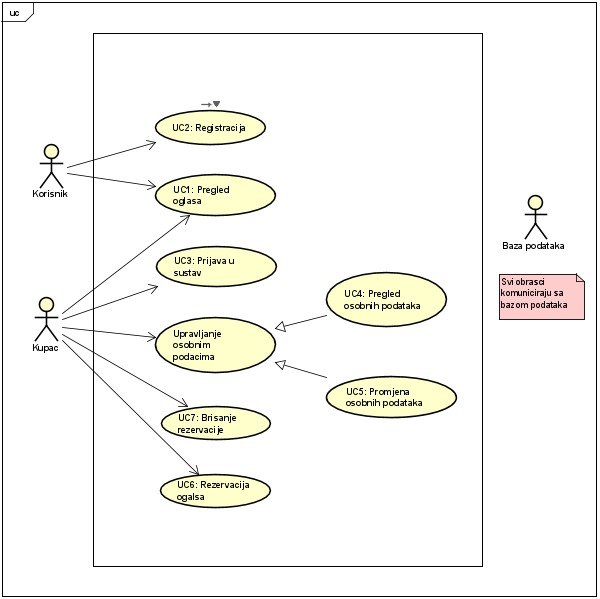
\includegraphics[scale=1]{dijagrami/DijagramOU1.PNG} %veličina slike u odnosu na originalnu datoteku i pozicija slike
						\centering
						\caption{ Dijagram obrasca uporabe, funkcionalnosti korisnika i kupca}
						\label{fig:dijagram1}
					\end{figure}
				
				
					\begin{figure}[H]
						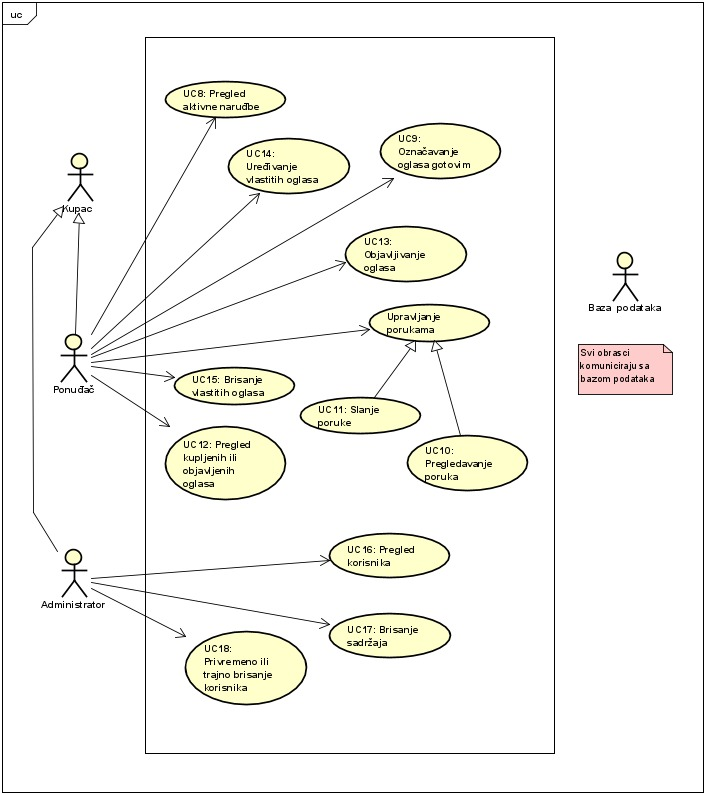
\includegraphics[scale=1]{dijagrami/DijagramOU2.PNG} %veličina slike u odnosu na originalnu datoteku i pozicija slike
						\centering
						\caption{ Dijagram obrasca uporabe, funkcionalnosti ponuđača i administratora}
						\label{fig:dijagram2}
					\end{figure}
				\eject		
				
			\subsection{Sekvencijski dijagrami}
				
				\textbf{UC6 - Rezervacija oglasa}

				Klijent salje zahtjev za prikaz svih oglasa. Posluzitelj dohvaca obliznje oglase i prikazuje ih. Odabirom oglasa,  posluzitelj iz baze podataka dohvaca osnovne podatke o oglasu i prikazuje ih korisniku. Da bi zapoceo rezervaciju, klijent salje zahtjev za rezervaciju. Posluzitelj u bazi podataka provjerava dostupnost oglasa. Ukoliko je oglas vec rezerviran, sustav obavjestava klijenta o tome uz poruku. Ako ogals nije rezerviran, posluzitelj informaciju o rezervaciji prosljeduje bazi koja sprema promjenu.
				
				\begin{figure}[H]
					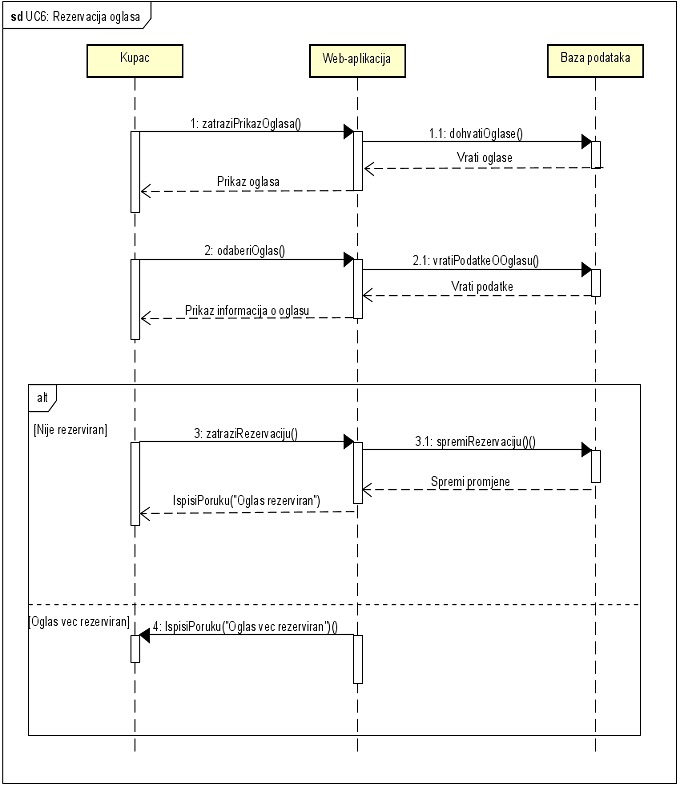
\includegraphics[scale=1]{dijagrami/SekvencijskiD.PNG} %veličina slike u odnosu na originalnu datoteku i pozicija slike
					\centering
					\caption{ Sekvencijski dijagram za UC6}
					\label{fig:dijagram3}
				\end{figure}
				\eject
	
		\section{Ostali zahtjevi}
		
		
			 
			 	\begin{itemize}
			 		\item Sustav treba omogućiti rad više korisnika u stvarnom vremenu
			 		
			 		\item Korisničko sučelje i sustav moraju podržavati hrvatsku abecedu (dijakritičke znakove) pri unosu i prikazu tekstualnog sadržaja
			 		
			 		
			 		\item  Izvršavanje dijela programa u kojem se pristupa bazi podataka ne smije trajati duže od nekoliko sekundi
			 		
			 		\item  Sustav treba biti implementiran kao web aplikacija koristeći objektno-orijentirane
			 		jezike
			 		
			 		\item  Neispravno korištenje korisničkog sučelja ne smije narušiti funkcionalnost i
			 		rad sustava
			 		
			 		\item  Sustav treba biti jednostavan za korištenje, korisnici se moraju znati koristiti
			 		sučeljem bez opširnih uputa
			 		
			 		\item  Nadogradnja sustava ne smije narušavati postojeće funkcionalnosti sustava
			 		
			 		\item  Sustav kao valutu koristi HRK
			 		
			 		\item  Veza s bazom podataka mora biti kvalitetno zaštićena, brza i otporna na vanjske greške
			 		
			 		\item  Pristup sustavu mora biti omogućen iz javne mreže pomoću HTTPS.
			 		
			 	\end{itemize}
	\chapter{Arhitektura i dizajn sustava}
		

		 Stil višeslojne arhitekture odjeljuje cjelovite komponente i te princip oblikovanja podijeli pa vladaj može preuzeti već postojeću podjelu. Troslojni stil arhitekture je prilagođen za jednostavne web aplikacije i mi ćemo ga koristiti za izradu naše aplikacije.
		 
		Arhitektura koju smo izabrali temelji se na principu oblikovanja podijeli pa vladaj. Tim principom smo uspjeli postići da odvojeni manji timovi unutar našeg tima rade na manjim problemima čime smo omogućili specijalizaciju. Takva podjela omogućuje efikasniji rad tima.
		
		\vspace{5mm}
		\noindent Arhitektura se sastoji od tri sloja:
		\begin{packed_enum}
			\item  podatkovni sloj
		
			\item  sloj poslovne logike
		
			\item  korisnički ili prezentacijski sloj
		\end{packed_enum}
	
	Podatkovni sloj je sloj za pohranu podataka u bazu ili datotečni sustav. U našoj aplikaciji koristit će se relacijska baza podataka, a odabrani jezik je SQL te razvojno okruženje PosgreSQL, pgAdmin . Također u početcima izrade aplikacije drugi slojevi će moći koristiti privremenu H2 bazu podataka pisanu u programskom jeziku Java u razvojom okruženju IntelliJIDEA.
	
	Sloj poslovne logike je sloj s implementacijom poslovnih procesa i izračuna. Kod web aplikacija ovaj sloj je podržan od strane web poslužitelja ili aplikacijskog poslužitelja. Ovaj sloj obrađuje i generira dinamički sadržaj koji prosljeđuje sljedećem sloju.
	
	Korisnički ili prezentacijski sloj je sloj s korisničkim sučeljem. Ovaj sloj kod web aplikacija se sastoji od web poslužitelja koji isporučuje statički i dinamički sadržaj, a sadržaj web stranice prikazuje web preglednik. Web poslužitelj to izvršava pomoću mrežnih protokola, a to su HTTP protokoli. Korisnik pomoću ovog sloja šalje upite i naredbe sloju poslovne logike koji ih obrađuje, te također pregledava sadržaj koji mu pruža sloj poslovne logike.

		Za razvoj naše aplikacije koristimo radni okvir Java Spring Boot. Pri korištenju tog radnog okvira potrebno je dodati još dodatnih slojeva u arhitekturu pri čemu se klijenstka i poslužiteljska strana mogu organizirati u više slojeva, ali ne utječu na organizaciju tima po glavna tri sloja.
		
		\vspace{5mm}
		\noindent Višeslojna se arhitektura u tom slučaju dijeli na šest slojeva:
		\begin{packed_enum}
			\item  sloj korisničke strane
		
			\item  sloj nadglednika
	
			\item  sloj usluge
		
			\item  sloj domene
		
			\item  sloj za pristup podatcima
		
			\item  sloj baze podataka
		\end{packed_enum}
		
	Sloj korisničke strane implementiran je u JavaScriptu, koristi React koji omogućuje prikaz korisničkog sučelja,a korištena paltforma je Microsoft visual studio.
	
	Sloj nadglednika povezuje korisničku stranu s poslužiteljskom stranom. Implementiran je u jeziku Java na platformi IntelliJIDEA.
	
	Sloj usluge obavlja svu poslovnu logiku i potrebne izračune. Implementiran je u jeziku Java na platformi IntelliJIDEA.
	
	Sloj domene ima razrađeni model podataka domene. Implementiran je u jeziku Java na platformi IntelliJIDEA.
	
	Sloj za pristup podatcima je sloj koji omogućuje spremanje i dohvat podataka iz određene baze podataka te razmjenu tih podataka sa slojem domene. Implementiran je u jeziku Java na platformi IntelliJIDEA.
	
	 Sloj baze podataka omogućuje pohranu podataka u relacijsku bazu ili H2 bazu. Za relacijsku bazu koriste se PostgreSQL i pgAdmin, a za H2 bazu koristi se Java na platformi IntelliJIDEA.
	
		

		

				
		\section{Baza podataka}
			
	  Naš sustav zahtijeva pohranu puno podataka, stoga je bilo potrebno izraditi relacijsku bazu podataka koju bi mogli koristiti za te potrebe. Baza nam je potrebna također za izmjenu i dohvat podataka za daljnju obradu te nam omogućava trajno čuvanje podataka. U ovoj ranijoj fazi izgradnje programske potpore za naš sustav odlučili smo se za jednostavniju verziju baze podataka H2 koja pohranjuje podatke u memoriju računala na kojemu je program pokrenut. U kasnijim fazama razvoja potpore ćemo se povezati na trajnu bazu podataka. Baza podataka koja nam je potrebna za naš sustav sastoji se od sljedećih entiteta:
		\begin{itemize}
			\item user
			\item address
			\item city
			\item role
			\item category
			\item ad
			\item condition
			\item message
			\item usersPrefersCategory
			\item adInCategory
			
		
		\end{itemize}
		
			\subsection{Opis tablica}
			
				\textbf{User	}
				Ovaj entitet modelira korisnika naše aplikacije. Entitet sadrži sljedeće atribute: idUser, userName, email, password, name, surname, idAdress i idRole. Atribut surname je opcionalan. Ovaj entitet je u vezi Many-to-One s entitetom Adress preko entiteta idAddress te u vezi Many-to-One s entitetom Role preko atributa idRole.
				
				\begin{longtabu} to \textwidth {|X[6, l]|X[6, l]|X[20, l]|}
					
					\hline \multicolumn{3}{|c|}{\textbf{User}}	 \\[3pt] \hline
					\endfirsthead
					
					\hline \multicolumn{3}{|c|}{\textbf{User}}	 \\[3pt] \hline
					\endhead
					
					\hline 
					\endlastfoot
					
					\cellcolor{LightGreen}\textbf{idUser} & INT	&  	Identifikacijski broj korisnika 	\\ \hline
					userName & VARCHAR	&  	Korisničko ime 	\\ \hline
					email	& VARCHAR &   Mail adresa korisnika	\\ \hline 
					password & VARCHAR & Lozinka korisnika  \\ \hline 
					name & VARCHAR	&  	Ime korisnika	\\ \hline 
					surname & VARCHAR	&  	Prezime korisnika	\\ \hline 
					
					\cellcolor{LightBlue}\textit{ idAdress}	& INT & Identifikacijski broj adrese korisnika   	\\ \hline 
					\cellcolor{LightBlue} \textit{ idRole}	& INT & Identifikacijski broj uloge korisnika   	\\ \hline 
					
					
				\end{longtabu}
				
				
				\textbf{Address		}
				Ovaj entitet predstavlja adresu našega korisnika. Sadrži atribute: idAddress, street, number, latitude, longitude i postalCode. Ovaj entitet u vezi je Many-to-One s entitetom City preko atributa postalCode.
				
				
				\begin{longtabu} to \textwidth {|X[6, l]|X[6, l]|X[20, l]|}
					
					\hline \multicolumn{3}{|c|}{\textbf{Address}}	 \\[3pt] \hline
					\endfirsthead
					
					\hline \multicolumn{3}{|c|}{\textbf{Address}}	 \\[3pt] \hline
					\endhead
					
					\hline 
					\endlastfoot
					
					\cellcolor{LightGreen}\textbf{idAddress}  & INT	&  	Identifikacijski broj adrese	\\ \hline
					street & VARCHAR	&  	Ulica lokacije 	\\ \hline
					number	& INT &  Kućni broj lokacije	\\ \hline 
					latitude & VARCHAR & Geografska širina lokacije \\ \hline 
					longitude & VARCHAR	&  Geografska duljina lokacije	\\ \hline 
					
					\cellcolor{LightBlue} \textit{  postalCode}	& INT & Poštanski broj mjesta u kojemu se nalazi \newline lokacija	\\ \hline  
					
					
				\end{longtabu}
				
				
			\textbf{City		}
				Ovaj entitet predstavlja grad unutar kojega živi naš korisnik. Sadrži atribute postalCode i cityName. 
				
				\begin{longtabu} to \textwidth {|X[6, l]|X[6, l]|X[20, l]|}
					
					\hline \multicolumn{3}{|c|}{\textbf{City}}	 \\[3pt] \hline
					\endfirsthead
					
					\hline \multicolumn{3}{|c|}{\textbf{City}}	 \\[3pt] \hline
					\endhead
					
					\hline 
					\endlastfoot
					
					\cellcolor{LightGreen} \textbf{postalCode} & INT	&  	Poštanski broj mjesta u kojemu se nalazi \newline lokacija	\\ \hline
					cityName & VARCHAR	&  Naziv grada u kojemu se nalazi lokacija 	\\ \hline			
					
				\end{longtabu}
				
				
				\textbf{Role		}
				Ovaj entitet predstavlja ulogu koju naš korisnik može imati. Sadrži atribute idRole i roleName.
				
				
				\begin{longtabu} to \textwidth {|X[6, l]|X[6, l]|X[20, l]|}
					
					\hline \multicolumn{3}{|c|}{\textbf{Role}}	 \\[3pt] \hline
					\endfirsthead
					
					\hline \multicolumn{3}{|c|}{\textbf{Role}}	 \\[3pt] \hline
					\endhead
					
					\hline 
					\endlastfoot
					
					\cellcolor{LightGreen} \textbf{idRole} & INT	&  	Identifikacijski broj uloge koju korisnik može \newline imati u sustavu	\\ \hline
					roleName & VARCHAR	&  	Naziv uloge  	\\ \hline
					
					
					
				\end{longtabu}
				
				
				\textbf{Category		}
				Ovaj entitet predstavlja kategoriju koju naš oglas može imati. Sadrži atribute idCategory te categoryName.
				
				
				\begin{longtabu} to \textwidth {|X[6, l]|X[6, l]|X[20, l]|}
					
					\hline \multicolumn{3}{|c|}{\textbf{Category}}	 \\[3pt] \hline
					\endfirsthead
					
					\hline \multicolumn{3}{|c|}{\textbf{Category}}	 \\[3pt] \hline
					\endhead
					
					\hline 
					\endlastfoot
					
					\cellcolor{LightGreen} \textbf{idCategory} & INT	&  	Identifikacijski broj kategorije	\\ \hline
					categoryName & VARCHAR	&  Naziv kategorije 	\\ \hline
										
				\end{longtabu}
		
		
		
		
				
				\textbf{Ad		}
				Ovaj entitet modelira oglas koji povezuje one koji žele prodati proizvod i one koji žele kupiti proizvod. Entitet sadrži atribute: idAd, caption, image, description, price, discount, timeOfAddition, timeOfExpiration, IdUserSeller, IdUserBuyer i  idCondition. Ovaj entitet u vezi je One-To-One s entitetom Condition preko idCondition, u vezi Many-to-One sa entitetom User preko atributa IdUserSeller te i preko atributa IdUserBuyer.
\begin{longtabu} to \textwidth {|X[10, l]|X[6, l]|X[20, l]|}
					
					\hline \multicolumn{3}{|c|}{\textbf{Ad}}	 \\[3pt] \hline
					\endfirsthead
					
					\hline \multicolumn{3}{|c|}{\textbf{Ad}}	 \\[3pt] \hline
					\endhead
					
					\hline 
					\endlastfoot
					
					\cellcolor{LightGreen} \textbf{idAd} & INT	&  	Identifikacijski broj oglasa	\\ \hline
					caption & VARCHAR	&  	Naslov oglasa 	\\ \hline
					image	& LONGBLOB &  Slika oglasa	\\ \hline 
					description & VARCHAR & Opis oglasa \\ \hline 
					price & DECIMAL	&  Cijena oglasa	\\ \hline 
					discount & INT	&  Popust koji se ostvaruje	\\ \hline 
					timeOfAddition & DATETIME	&  Vrijeme postavljanja oglasa	\\ \hline 
					timeOfExpiration & DATETIME	&  Vrijeme trajanja oglasa	\\ \hline 
					
					\cellcolor{LightBlue} \textit{  IdUserSeller}	& INT & Identifikacijski broj korisnila koji je \newline objavio oglas	\\ \hline  
					\cellcolor{LightBlue} \textit{  IdUserBuyer}	& INT & Identifikacijski broj korisnila koji je \newline kupio preko oglas	\\ \hline  
					\cellcolor{LightBlue} \textit{  idCondition}	& INT & Identifikacijski broj stanja oglasa\\ \hline  
					
					
				\end{longtabu}
				
				
				
				
				\textbf{Condition 		}
				Ovaj entitet predstavlja  stanje u kojemu se nalazi oglas. Entitet sadrži atribute: idCondition i conditionName.
				
				\begin{longtabu} to \textwidth {|X[8, l]|X[6, l]|X[20, l]|}
					
					\hline \multicolumn{3}{|c|}{\textbf{Condition}}	 \\[3pt] \hline
					\endfirsthead
					
					\hline \multicolumn{3}{|c|}{\textbf{Condition}}	 \\[3pt] \hline
					\endhead
					
					\hline 
					\endlastfoot
					
					\cellcolor{LightGreen} \textbf{idCondition} & INT	&  	Identifikacijski broj stanja	\\ \hline
					conditionName & VARCHAR	&  	Naziv stanja \\ \hline
					
					
				\end{longtabu}
				
				
				
				
				\textbf{Message 		}
				Ovaj entitet modelira poruke koje izmjenuju kupac i prodavač. Entitet sadrži atribute: idMessage, text, time, idUserRecieved i idUserSent. Entitet je u vezi Many-to-One sa entitetom User preko atributa idUserSent i atributa idUserRecieved.
				
				
				\begin{longtabu} to \textwidth {|X[8, l]|X[6, l]|X[20, l]|}
					
					\hline \multicolumn{3}{|c|}{\textbf{Message}}	 \\[3pt] \hline
					\endfirsthead
					
					\hline \multicolumn{3}{|c|}{\textbf{Message}}	 \\[3pt] \hline
					\endhead
					
					\hline 
					\endlastfoot
					
					\cellcolor{LightGreen} \textbf{idMessage} & INT	&  	Identifikacijski broj poruke\\ \hline
					text & VARCHAR	&  	Tekst poruke 	\\ \hline
					time	& DATETIME &  Vrijeme poruke	\\ \hline 
					
					\cellcolor{LightBlue} \textit{  idUserRecieved}	& INT & Identifikacijski broj korisnika koji je dobio \newline poruku	\\ \hline  
					\cellcolor{LightBlue} \textit{  idUserSent}	& INT & Identifikacijski broj korisnika koji je poslao \newline poruku	\\ \hline  
					
					
				\end{longtabu}
				
				
				\textbf{UsersPrefersCategory 		}
				Ovaj entitet sadrži podatke koji nam govore koje su korisniku najdraže kategorije oglasa. Entitet sadrži atribute: idUser i idCategory. Entitet je u vezi Many-to-Many sa entitetom User preko atributa idUser te je u vezi Many-to-Many sa entitetom Category preko atributa idCategory.
				
				\begin{longtabu} to \textwidth {|X[6, l]|X[6, l]|X[20, l]|}
					
					\hline \multicolumn{3}{|c|}{\textbf{UsersPrefersCategory}}	 \\[3pt] \hline
					\endfirsthead
					
					\hline \multicolumn{3}{|c|}{\textbf{UsersPrefersCategory}}	 \\[3pt] \hline
					\endhead
					
					\hline 
					\endlastfoot
					
					\cellcolor{LightGreen} \textbf{idUser} & INT	&  	Identifikacijski broj korisnika 	\\ \hline
					
					\cellcolor{LightBlue} \textit{  idCategory}	& INT & Identifikacijski broj kategorija koje korisnik \newline preferira	\\ \hline  
					
					
				\end{longtabu}
				
				
				
				\textbf{AdInCategory 		}
				Ovaj entitet sadrži podatke koji nam govore koje sve kategorije mogu biti oglasi. Entitet sadrži atribute: idAd i idCategory. Entitet je u vezi Many-to-Many sa entitetom Ad preko atributa idAd te je u vezi Many-to-Many sa entitetom Category preko atributa idCategory.
				
				
				\begin{longtabu} to \textwidth {|X[6, l]|X[6, l]|X[20, l]|}
					
					\hline \multicolumn{3}{|c|}{\textbf{AdInCategory}}	 \\[3pt] \hline
					\endfirsthead
					
					\hline \multicolumn{3}{|c|}{\textbf{AdInCategory}}	 \\[3pt] \hline
					\endhead
					
					\hline 
					\endlastfoot
					
					\cellcolor{LightGreen} \textbf{idAd} & INT	&  	Identifikacijski broj oglasa	\\ \hline
					
					\cellcolor{LightBlue} \textit{  idCategory}	& INT & Identifikacijski broj kategorije oglasa	\\ \hline  
					
					
				\end{longtabu}
				
			
			\subsection{Dijagram baze podataka}
			
				\begin{figure}[H]
			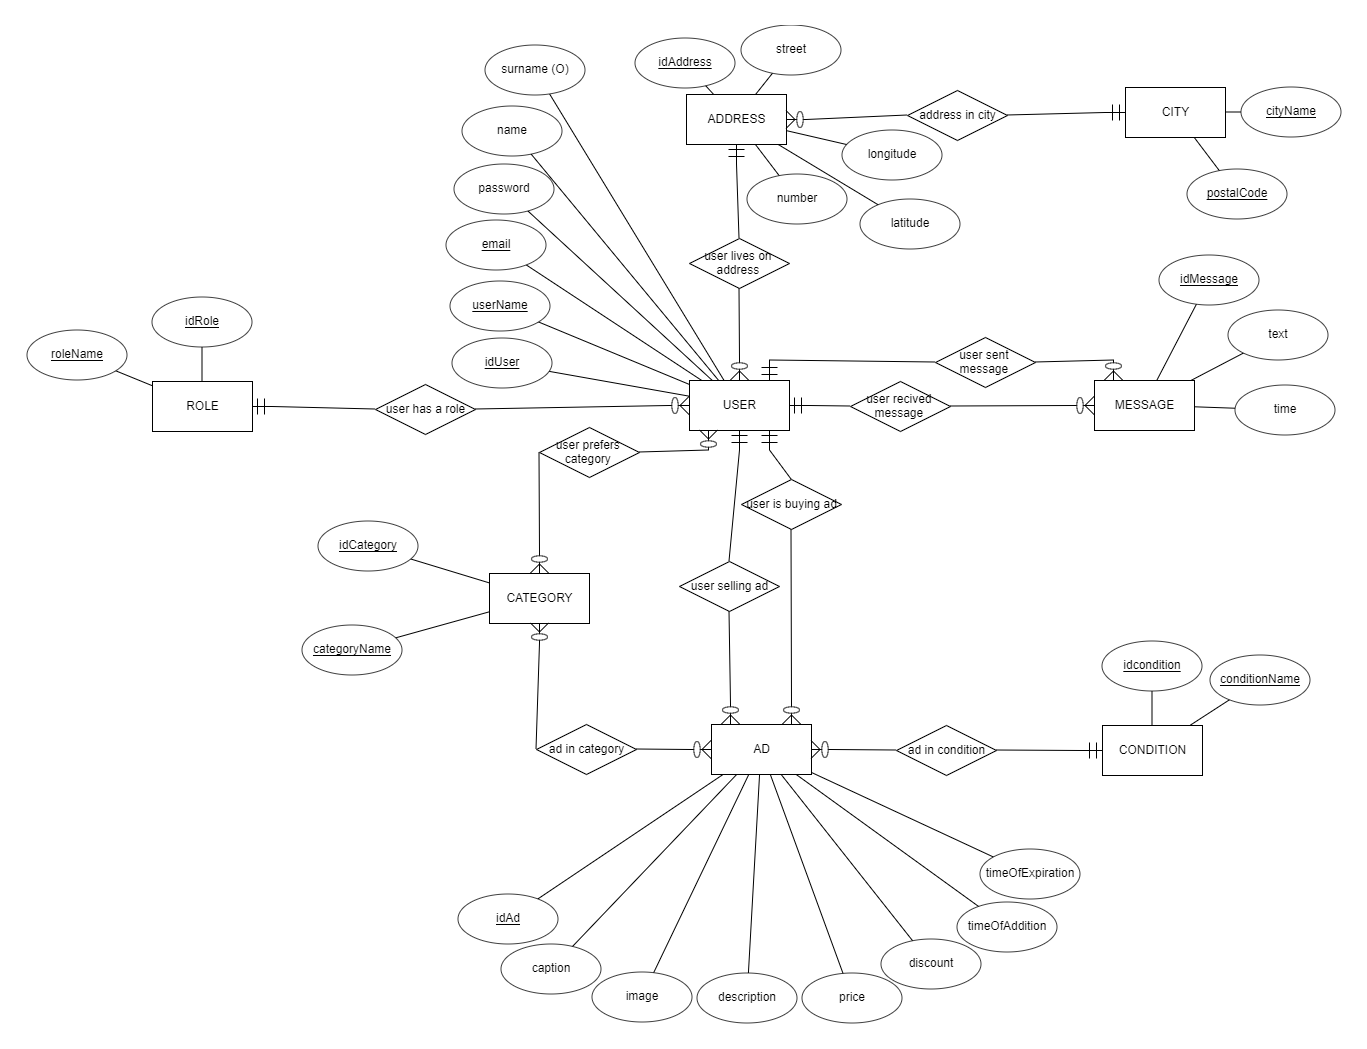
\includegraphics[scale=0.3]{slike/DatabaseER.PNG} %veličina slike u odnosu na originalnu datoteku i pozicija slike
			\centering
			\caption{E-R dijagram baze podataka}
			\label{fig:dijagramBaze1}
		\end{figure}
	
	\begin{figure}[H]
		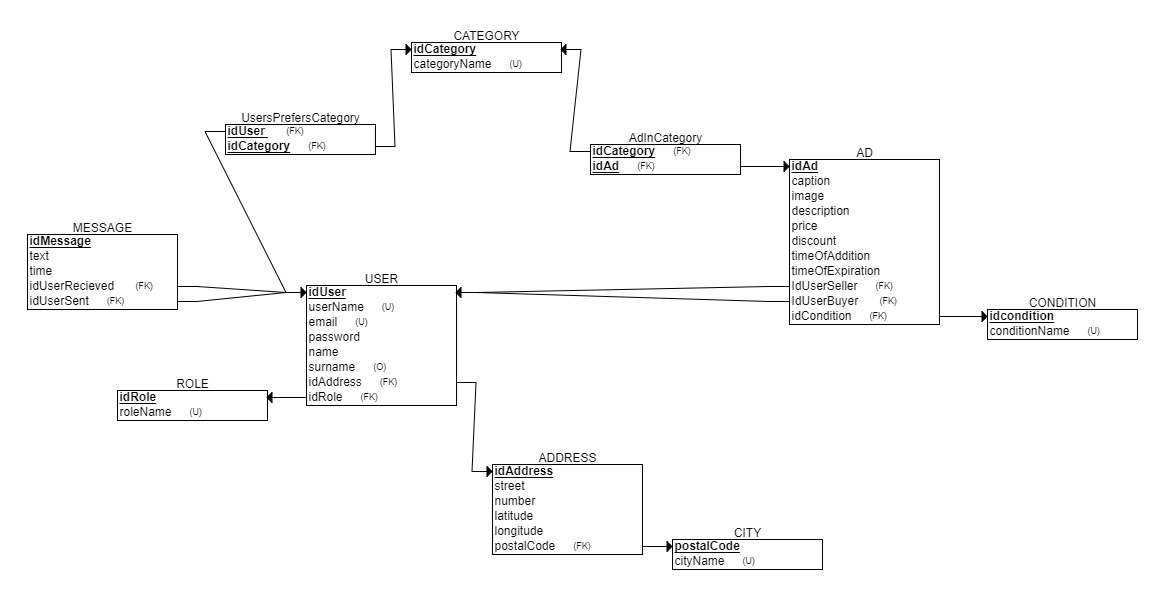
\includegraphics[scale=0.4]{slike/DijagramBaze.PNG} %veličina slike u odnosu na originalnu datoteku i pozicija slike
		\centering
		\caption{Relacijski dijagram baze podataka}
		\label{fig:dijagramBaze2}
	\end{figure}
			\eject
			
		\section{Dijagram razreda}
		
		Na slikama su prikazani razredi koji pripadaju backend dijelu arhitekture. Prva slika prikazuje razred UserController i AuthController koji nasljeđuju razred Contoller. Metode implementirane u tim razredima manipuliraju s DTO(Data transfer object) , a oni su dohvaćeni pomoću metoda implementiranih u Model razredima.
		
			
			\begin{figure}[H]
				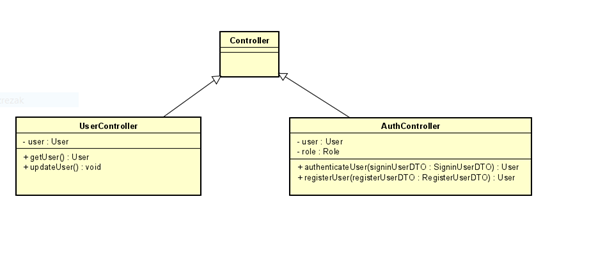
\includegraphics[scale=1]{slike/DijagramRazredaC.PNG} %veličina slike u odnosu na originalnu datoteku i pozicija slike
				\centering
				\caption{Dijagram razreda - Controllers}
				\label{fig:dijagramRazredaC}
			\end{figure}
		
			\begin{figure}[H]
				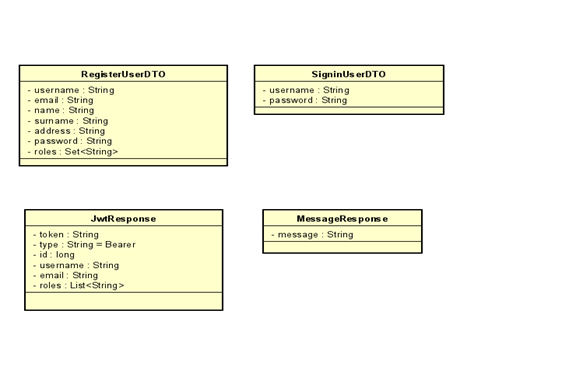
\includegraphics[scale=1]{slike/DijagramRazredaD.PNG} %veličina slike u odnosu na originalnu datoteku i pozicija slike
				\centering
				\caption{Dijagram razreda - DTO}
				\label{fig:dijagramRazredaC}
			\end{figure}
	
	
			\begin{figure}[H]
				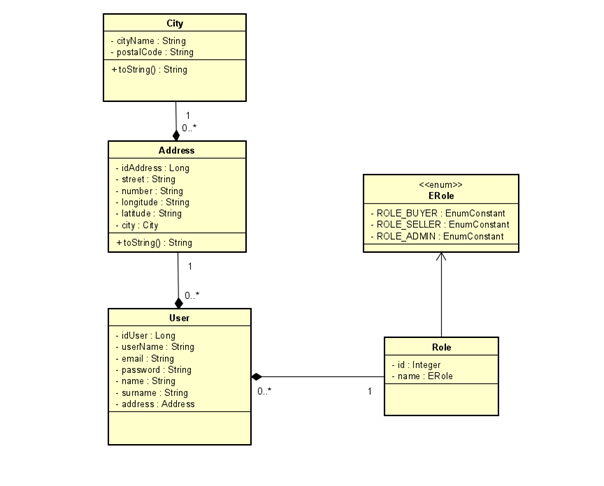
\includegraphics[scale=1]{slike/DijagramRazredaM.PNG} %veličina slike u odnosu na originalnu datoteku i pozicija slike
				\centering
				\caption{Dijagram razreda - Models}
				\label{fig:dijagramRazredaC}
			\end{figure}
			
			\eject
			
			\section{Dijagram stanja}
			
				\textbf{\textit{}}\\
			
Dijagram stanja prikazuje stanja objekta te prijelaze iz jednog stanja u drugo temeljene na dogadajima. Na slici ispod prikazan je dijagram stanja za prijavljenog korisnika koji samo kupuje ono što drugi korisnici objave.Kada se kupac prijavi, otvara mu se početna strana na kojoj vidi trenutne aktivne oglase. Također tu može pretražiti oglase po svome izboru te može rezervirati željene oglase. Ukoliko klikne na "Profil" otvaraju mu se svi trenutni podatci te ih može urediti. Ukoliko se odluči za "Poruke" tamo može pregledati sve primljene i poslane poruke. Ukoliko klikne na gumb "Moji oglasi" tamo može pregledati i pretražiti rezervirane i kupljene oglase. Konačno ako pritisne gumb "Odjavi", korisnik se odjavljuje te mu se prikazuje stranica za prijavu.

			\begin{figure}[H]
				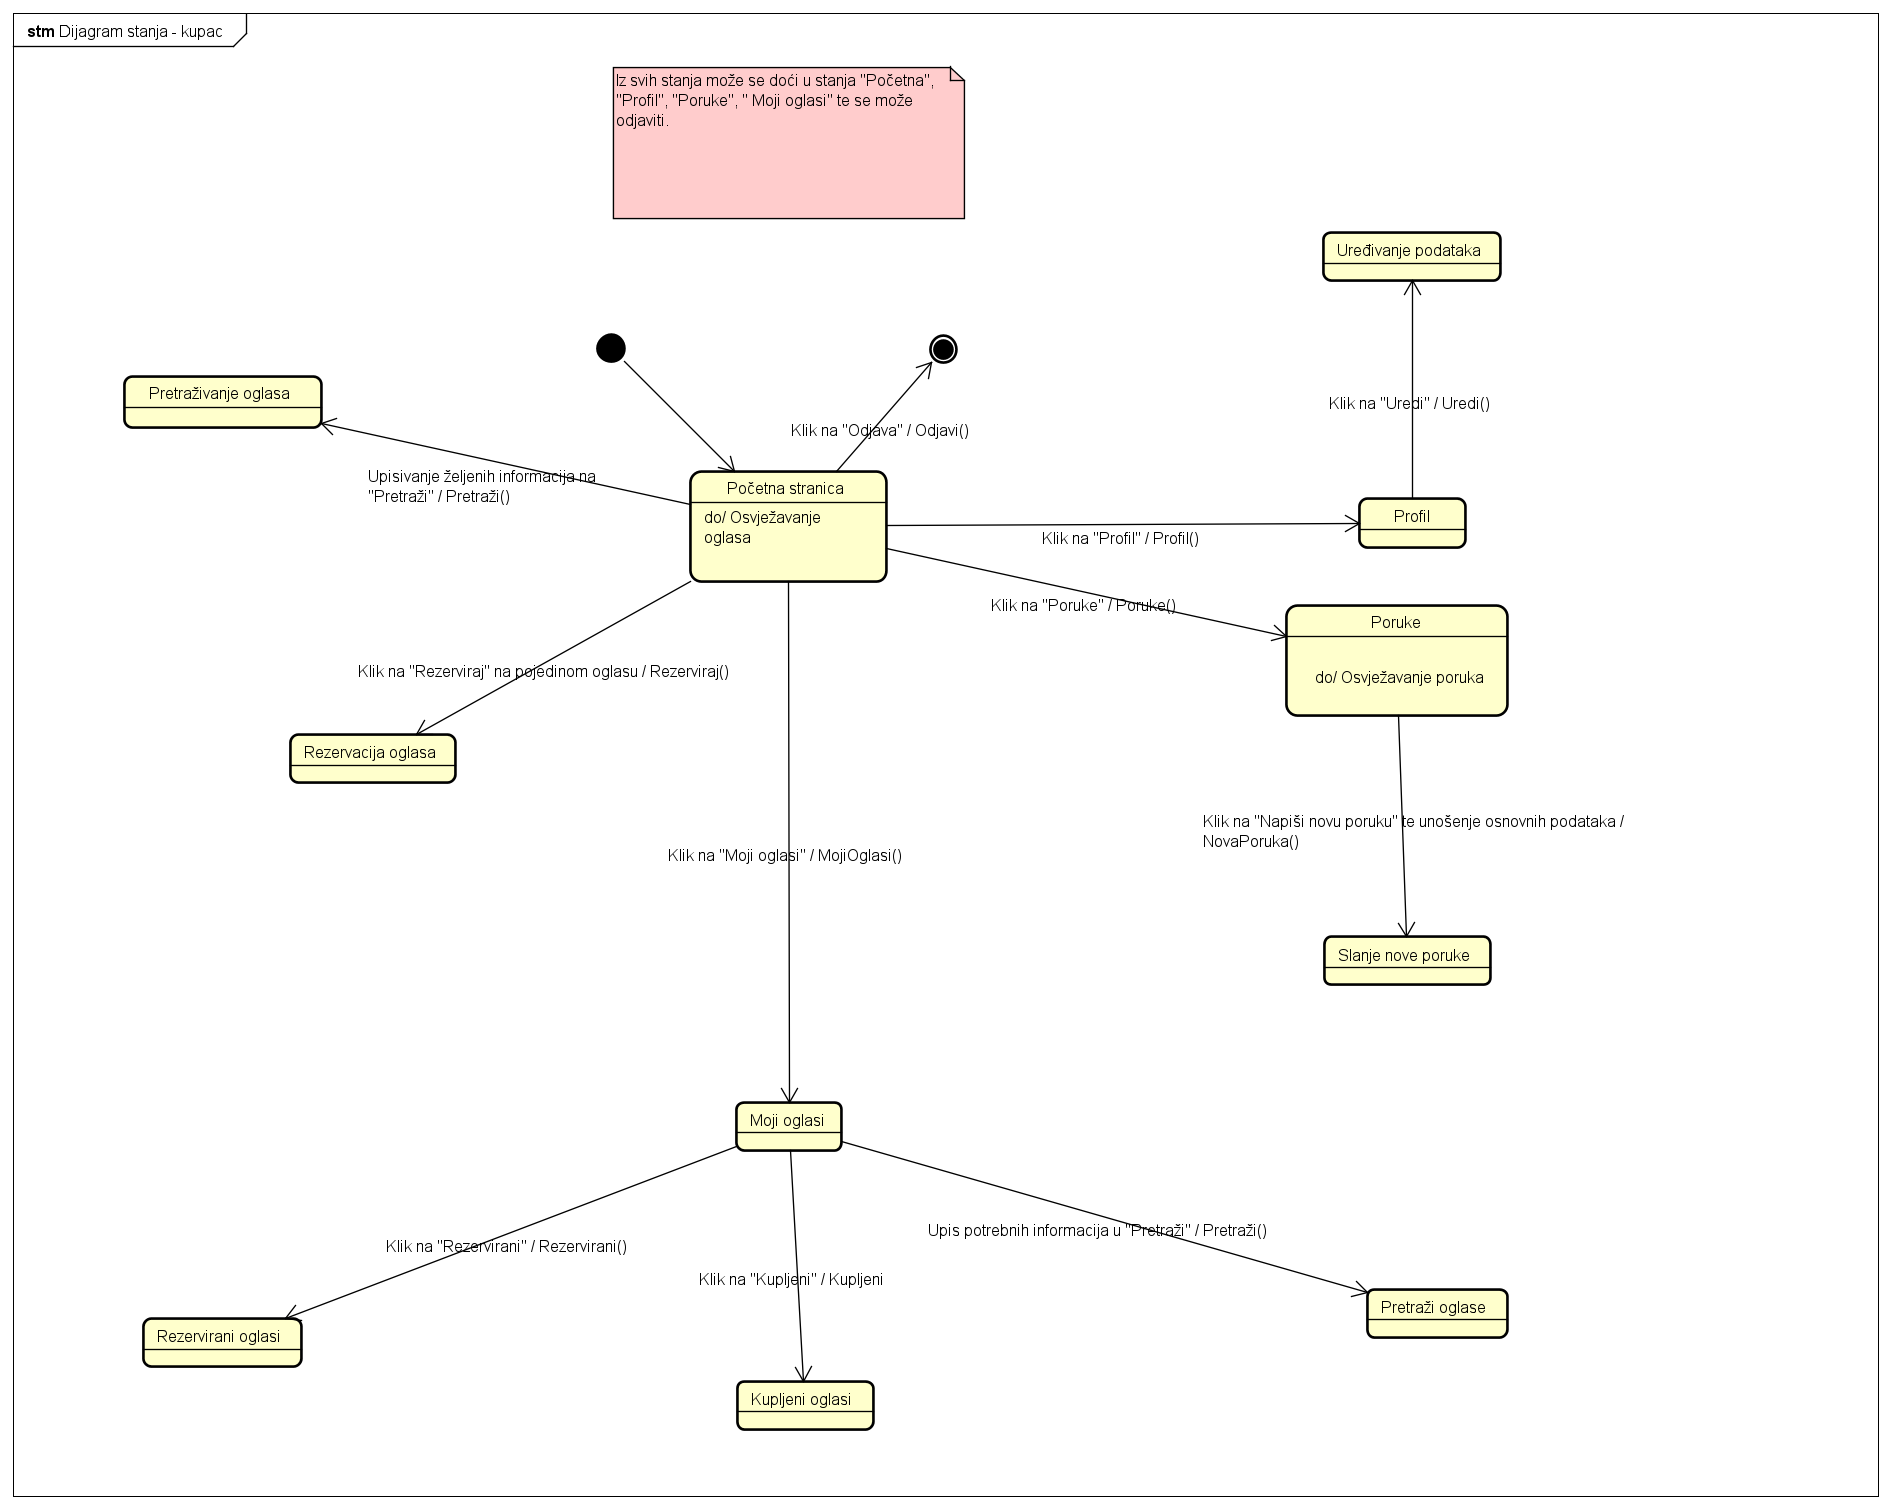
\includegraphics[scale=0.3]{slike/Dijagram_stanja_kupac.PNG} %veličina slike u odnosu na originalnu datoteku i pozicija slike
				\centering
				\caption{Dijagram stanja}
				\label{fig:dijagramStanja}
			\end{figure}
			
			
			\eject 
			
			\section{Dijagram aktivnosti}
			
			\textbf{\textit{dio 2. revizije}}\\
			
			\textit{Potrebno je priložiti dijagram aktivnosti s pripadajućim opisom. Dijagram aktivnosti treba prikazivati značajan dio sustava.}
			
			\eject
			\section{Dijagram komponenti}
			
			\textbf{\textit{dio 2. revizije}}\\
			
			\textit{Potrebno je priložiti dijagram komponenti s pripadajućim opisom. Dijagram komponenti treba prikazivati strukturu cijele aplikacije.}
		

	%\chapter{Implementacija i korisničko sučelje}
		
		
		\section{Korištene tehnologije i alati}
		
			\textbf{\textit{}}
			
Komunikacija unutar tima:
\vspace{4mm}
	
WhatsApp

Komunikacija unutar tima ostvarena je korištenjem aplikacije WhatsApp. 
WhatsApp je aplikacija za komunikaciju korisnika. Omogućava komunikaciju u stvarnom vremenu putem tekstualnih poruka, glasovnih poruka ili videopoziva. Podržava mogućnost dijeljenja slika, dokumenata i videa.

Službena stranica: https://www.whatsapp.com/
\vspace{3mm}

Microsoft Teams

Video sastanci tima, zajedničko uređivanje i diejljenje dokumenata održavani su putem aplikacije Microsoft Teams. 
Microsoft Teams je aplikacija koja nudi radni prostor timovima u obliku videokonferencija, poruka, pohrane datoteka i zajedničkog uređivanja dokumenata u stvarnom vremenu. 

Službena stranica: https://www.microsoft.com/hr-hr/microsoft-365/microsoft-teams/group-chat-software

\vspace{8mm}
Dokumentacija:
\vspace{4mm}

Astah UML 

Za izradu svih UML dijagrama korišten je Astah UML.
Astah UML je alat za stvaranje UML dijagrama. Omogućava stvaranje  dijagrama obrazaca uporabe, dijagrama razreda, dijagrama stanja, dijagrama aktivnosti, sekvencijskih dijagrama, dijagrama komponenata, dijagrama komunikacije, složene strukture, razmještaja i umnih mapa. 

Službena stranica: https://astah.net
\vspace{3mm}

Texmaker

Za pisanje dokumentacije koristili smo Texmaker.
Texmaker je besplatni višeplatformski LaTeX uređivač. Uključuje mnoge alate potrebne za razvoj dokumenata s LaTeX-om, podršku za unicode, provjeru pravopisa, automatsko dovršavanje i ugrađeni pdf preglednik.

Službena stranica: https://www.xm1math.net/texmaker/
\vspace{8mm}

Rad na aplikaciji:
\vspace{4mm}

Git i GitLab

Git je korišten kao sustav za upravljanje izvornim kodom, dok je udaljeni reozitorij projekta dostupan na web platformi GitLab.
Git je sustav otvorenog koda namijenjen upravljanju izvornim kodom. Pruža podršku za razvoj, stvaranje i spajanje grana.
GitLab je web platforma koja pruža upravljanje Git repozirotijem i kontinuiranu integraciju uz praćenje verzija. 

Službene stranice: https://git-scm.com/

	https://gitlab.com/
\vspace{3mm}

H2

Kao početna baza podataka koristio se H2 sustav.
H2 je sustav za upravljanje relacijskom bazom podataka napisanom u programskom jeziku Java. Omogućava čuvanje svih podataka u memoriji i podaci se osvježavaju pri svakom pokretanju aplikacije.

Službena stranica:https://www.h2database.com/html/main.html 
\vspace{3mm}

PostgreSQL i pgAdmin

Stalna baza u aplikaciji izrađena je pomoću PostgreSQL u pgAdminu.
PostgreSQL je bespaltan sustav otvorenog koda za upravljanje relacijskom bazom podataka. Podržava SQL upite i provjerava sigurnost.
PgAdmin je bespaltni administratorki alat s grafičkim korisničkim sučeljem za upravljanje PostgreSQL-om.

Službena stranica: https://www.pgadmin.org/
\vspace{3mm}

Intellij IDEA

Za pisanje koda korišten je Intellij IDEA
Intellij IDEA je integrirana razvojna okolina za razvoj programske potpore. Sadrži integrirani sustav za upravljanje inačicama. Najpopularnija razvojna okolina za pisanje programske potpore u programskom jeziku Java.

Službena stranica: https://www.jetbrains.com/idea/
\vspace{3mm}


HTML

Za prikaz web aplikacije koristi se HTML. 
HTML je standardni označni jezik i u njemu se pišu dokumenti koji se prikazuju u web pregledniku. Opisuje semantičku strukturu web stranice.
\vspace{3mm}

CSS

Stilska prezentacija web stranice izvdena je pomoću CSS-a.
CSS je stilski jezik za opis prezentacije dokumenta napisanog u označnom jeziku i omogućava odvajanje sadržaja od prezentacije što omogućava veću fleksibilnost pri izradi. 

\vspace{8mm}
Za izradu fronteda koristili smo React i JavaScript. 
\vspace{4mm}

JavaScript

Dinamičko kreiranje web stranice izvedeno je pomoću JavaScript-a. JavaScript je skriptni programski jezik koji se izvršava u internet pregledniku
na strani korisnika.

Službena stranica: https://www.javascript.com/
\vspace{3mm}

React

React je biblioteka u JavaScriptu za izgradnju korisničkih sučelja. Održavana je od strane Facebooka. 
React se najčešće koristi kao osnova u razvoju web ili mobilnih aplikacija. 

Službena stranica: https://reactjs.org/
\vspace{3mm}

SpringBoot

Za izradu pozadinske aplikacije(engl. back-end) koristili smo SpringBoot. Pozadinska aplikacija pisana je u razvojnom okruženju IntelliJ, koje je
omogućilo korištenje okvira Spring Boot koji je baziran na programskom jeziku Java. Spring Boot je projekt koji se oslanja na Spring Framework i koji omogućuje puno učinkovitiji i brži pristup izgradnji Spring aplikacija.

Službena stranica: https://spring.io/projects/spring-boot
\vspace{5mm}

			
			
			\eject 
		
	
		\section{Ispitivanje programskog rješenja}
			
		Provedeno je ispitivanje programskog rješenja u svrhu pronalaska grešaka i nepredviđenog ponašanja sustava na korisnikove akcije. Testiranje se sastoji od da dijela, testiranja komponenti sustava te testiranje sustava u cjelini. U svrhu testiranja komponenti programskog rješenja korišten je alat JUnit. Ponašanje sustava je testirano pomoću alata Selenium WebDriver za Google Chrome
			
			\subsection{Ispitivanje komponenti}
			Ispitivanjem komponenti testirana je funkcionalnost razreda koji implementiraju temeljne funkcionalnosti sustava.
			
			\textbf{Ispitni slučaj 1: Testiranje dohvata podataka o korisniku iz baze podataka premu username-u}
			
			Testira se dohvaća li metoda findByUsername(String username) doista korisnika čije smo podatke zapisali u bazu podataka.
			
			
			
			\begin{figure}[H]
				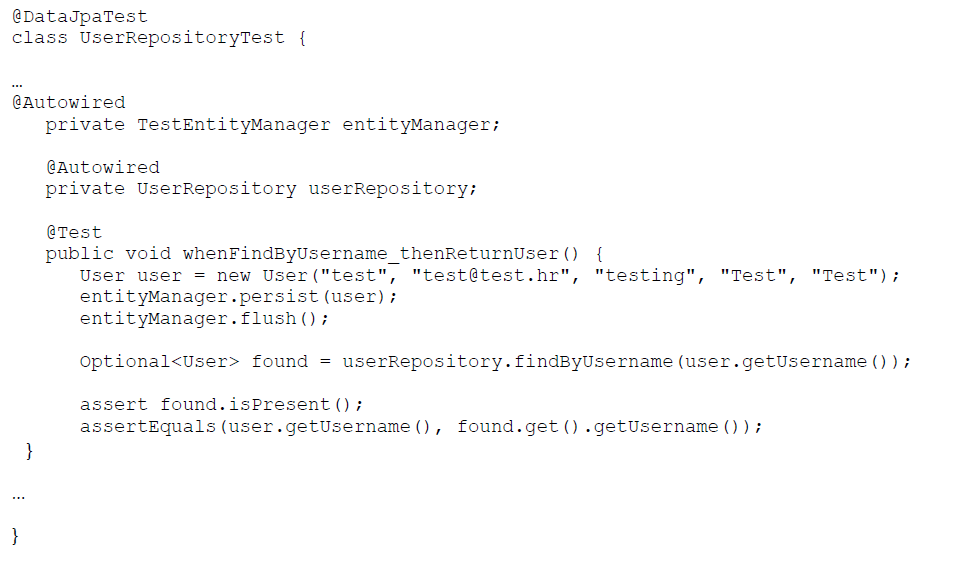
\includegraphics[scale=0.7]{slike/test1.PNG} %veličina slike u odnosu na originalnu datoteku i pozicija slike
				\centering
				\caption{Testiranje dohvata korisnika po username-ui}
				\label{fig:test1}
			\end{figure}
			
			
			
			
			
				\textbf{Ispitni slučaj 2: Testiranje postoji li korisnik u bazi podataka po username-u}
				
			Testira se funkionalnost metode findByUsername(String username) tako da se pomoću metode existsByUsername(String username) provjerava postoji li korisnik u bazi podataka ako postoji da će
			metoda findByUsername(String username) također pronaći zapis u korisniku u bazi podataka, u suprotnom nijedna od navedenih metoda neće pronaći podatke o korisniku.
				
				
				\begin{figure}[H]
					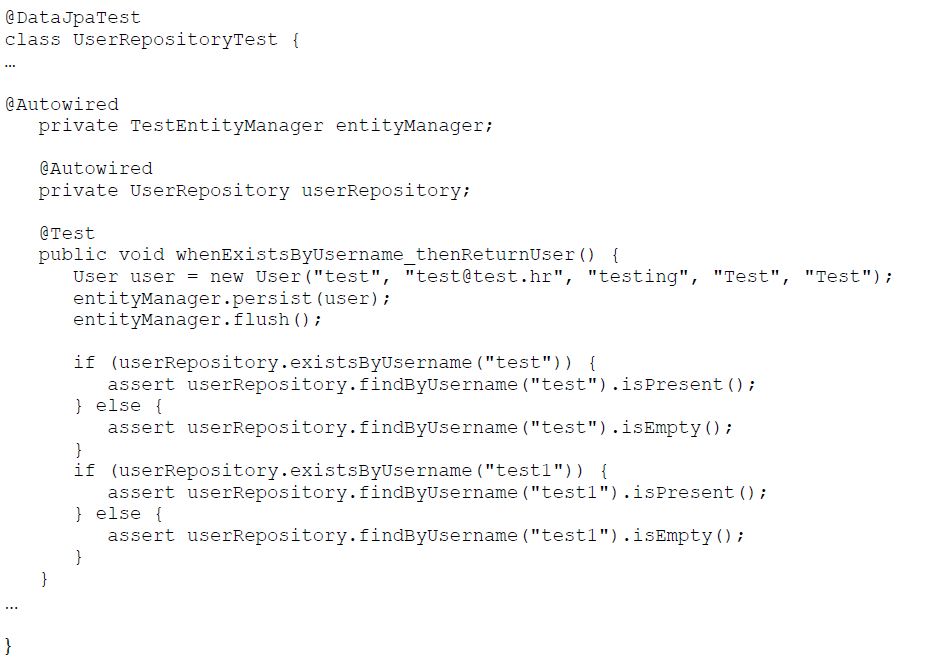
\includegraphics[scale=0.7]{slike/test2.PNG} %veličina slike u odnosu na originalnu datoteku i pozicija slike
					\centering
					\caption{Testiranje postoji li korisnik u bazi podataka po username-u}
					\label{fig:test2}
				\end{figure}
			
			\textbf{Ispitni slučaj 3: Testiranje postoji li korisnik u bazi podataka po email-u}
			
		Testira se funkionalnost metode findByEmail(String email) tako da se pomoću metode existsByEmail(String email) provjerava postoji li korisnik u bazi podataka te ako postoji da će metoda findByEmail(String email) također pronaći zapis o korisniku u bazi podatak, u suprotnom nijedna od navedenih metoda neće pronaći podatke o korisniku.
			
			\begin{figure}[H]
				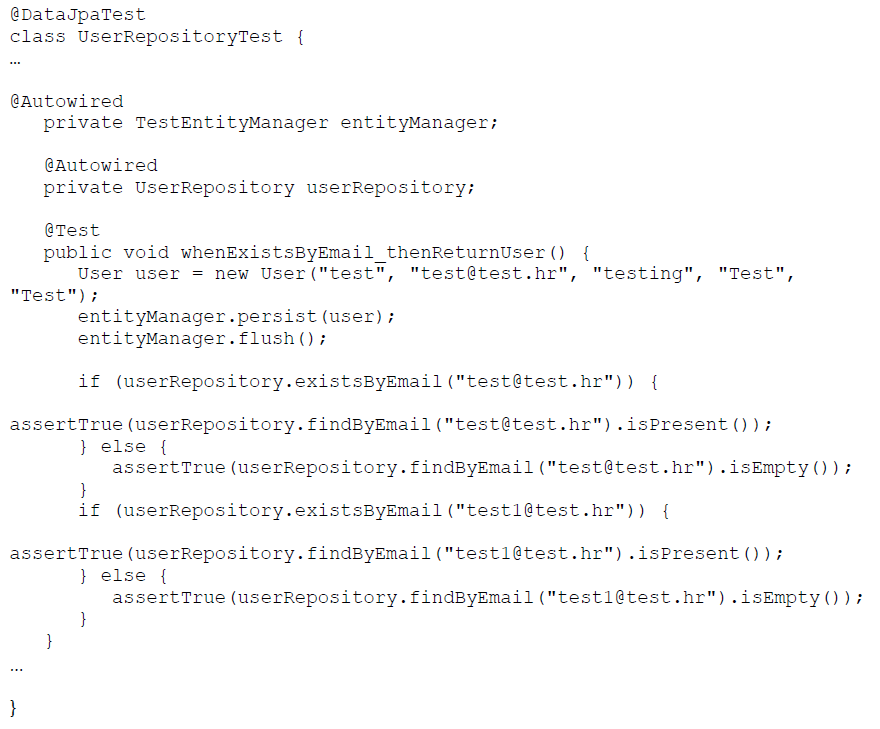
\includegraphics[scale=0.7]{slike/test3.PNG} %veličina slike u odnosu na originalnu datoteku i pozicija slike
				\centering
				\caption{Testiranje postoji li korisnik u bazi podataka po email-u}
				\label{fig:test3}
			\end{figure}
		
		U svrhu sljedećih ispitivanja koriste se dvojnici odnosno Mock objekti kojima možemo simulirati radi stavrnih objekata
		
		\begin{figure}[H]
			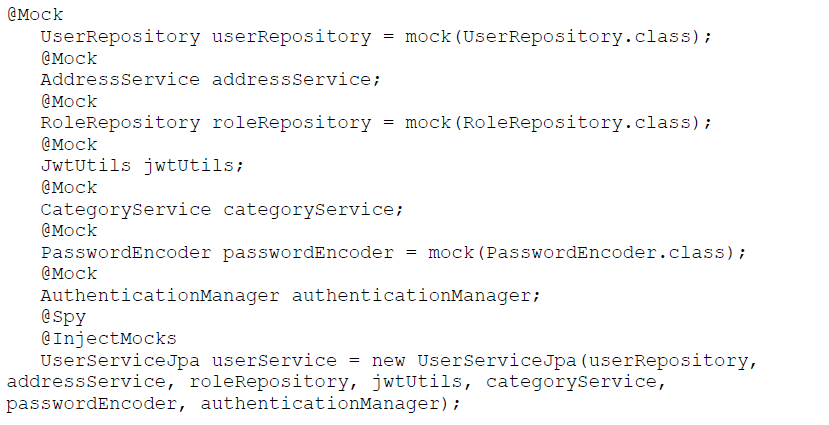
\includegraphics[scale=0.7]{slike/test3a.PNG} %veličina slike u odnosu na originalnu datoteku i pozicija slike
			\centering
			\caption{Mock objekti}
			\label{fig:test3a}
		\end{figure}
		
		
		\textbf{Ispitni slučaj 4: Testiranje registracije}
		Testiramo dobivamo li za povratnu vrijednost metode za registraciju korisnika doista korisnika kojeg smo htjeli registrirati.
		
		
		\begin{figure}[H]
			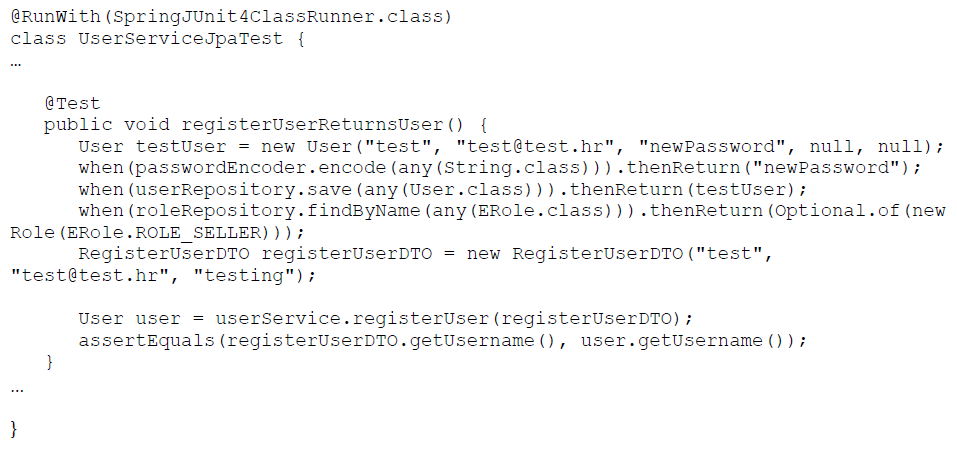
\includegraphics[scale=0.7]{slike/test4.PNG} %veličina slike u odnosu na originalnu datoteku i pozicija slike
			\centering
			\caption{Testiranje registracije korisnika}
			\label{fig:test4}
		\end{figure}
	
	\textbf{Ispitni slučaj 5 : Testiranje jedinstvenosti email-a}
	
	Testiramo mogu li se registrirati dva korisnika s identičnom email adresom, očekivano ponašanje je bacanje iznimke RequestDeniedException. 
	
	\begin{figure}[H]
		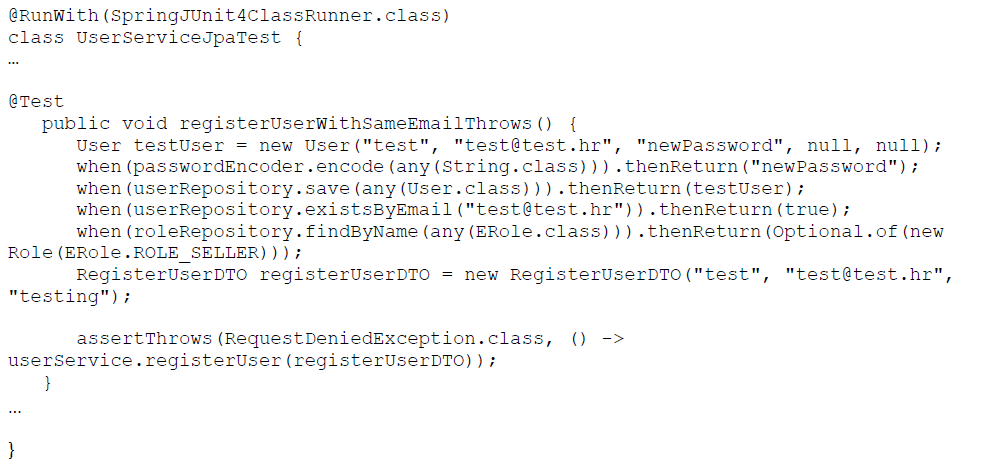
\includegraphics[scale=0.7]{slike/test5.PNG} %veličina slike u odnosu na originalnu datoteku i pozicija slike
		\centering
		\caption{Testiranje jedinstvenosti email-a}
		\label{fig:test5}
	\end{figure}
			
			
				\textbf{Ispitni slučaj 6 : Testiranje jedinstvenosti username-a}
			
		Testiramo mogu li se registrirati dva korisnika s identičnim korisničkim imenom, očekivano ponašanje je bacanje iznimke RequestDeniedException. 
			
			\begin{figure}[H]
				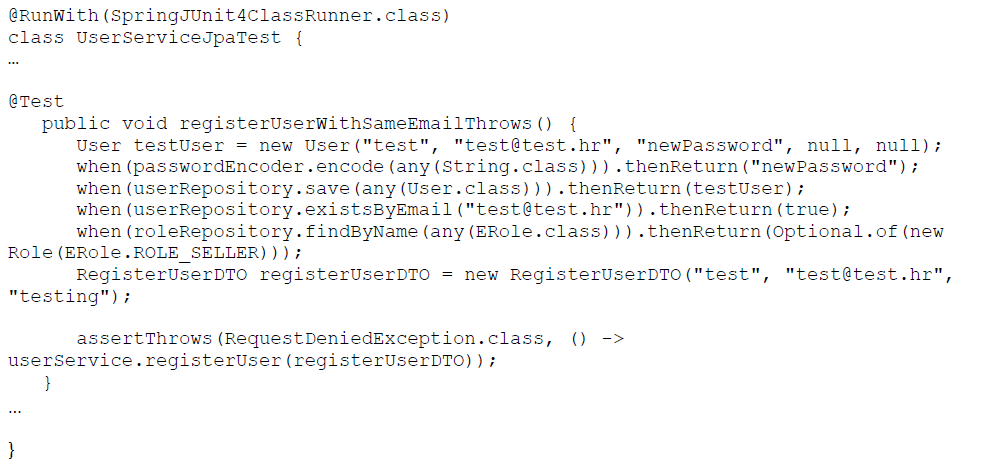
\includegraphics[scale=0.7]{slike/test5.PNG} %veličina slike u odnosu na originalnu datoteku i pozicija slike
				\centering
				\caption{Testiranje jedinstvenosti username-a}
				\label{fig:test6}
			\end{figure} 
		
			\subsection{Ispitivanje sustava}
			
			
			Ispitivanje sustava je provedeno pomoću alata Selenium WebDriver za web preglednik Google Chrome. Testirani su slučajevi registracije i prijave korisnika te objava oglasa, rezervacija oglasa i slanje poruka.
			
			
			\textbf{Ispitni slučaj 1: Ispitivanje registrcije}
			
		Pomoću konfiguriranog Chreome drivrera dohvaća se stranica za registraciju i šalju se potrebni podatci za registraciju korisnika, prvim izvođenjem testa email korisnika i korisničko ime su jedinstveni te je očekivani rezultat uspješna registracija.
			
			
			
			\begin{figure}[H]
				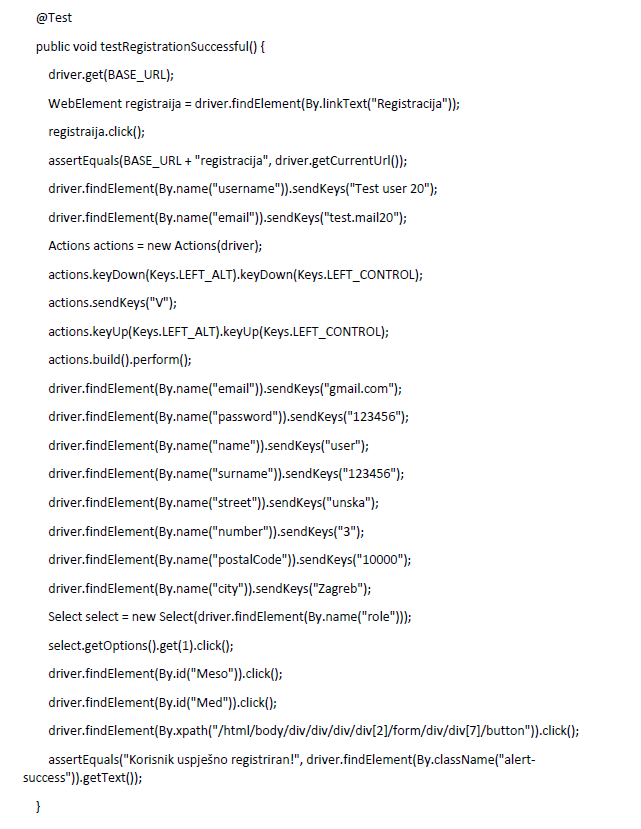
\includegraphics[scale=0.9]{slike/sel1.PNG} %veličina slike u odnosu na originalnu datoteku i pozicija slike
				\centering
				\caption{Testiranje registracije}
				\label{fig:sel1}
			\end{figure}
			
			
			
			
			
			\textbf{Ispitni slučaj 2: Testiranje prijave postojećeg korisnika
				}
			
			Testiramo prijavu u aplikaciju pomoću unaprijed registriranog korisnika, očekivano ponašanje je uspješna prijava što dokazujemo ispisivanje korisničkog imena prijavljenog korisnika u gornjem desnom kutu stranice.
			
			
			\begin{figure}[H]
				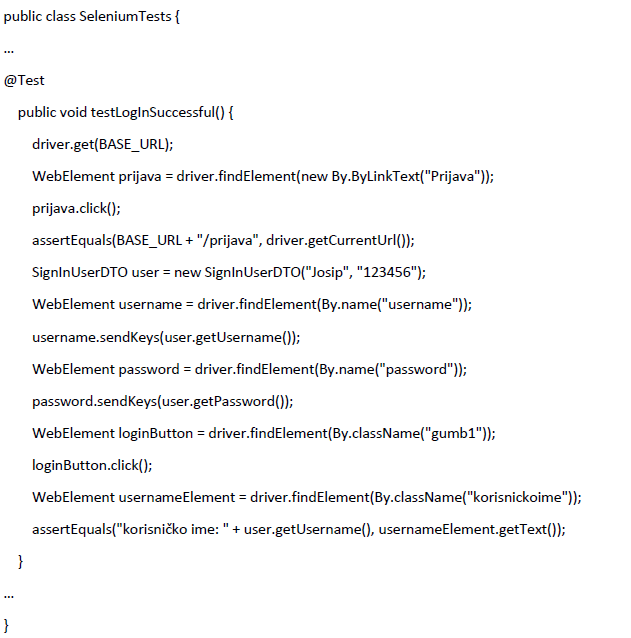
\includegraphics[scale=0.9]{slike/sel2.PNG} %veličina slike u odnosu na originalnu datoteku i pozicija slike
				\centering
				\caption{Testiranje prijave postojećeg korisnika}
				\label{fig:sel2}
			\end{figure}
			
			\textbf{Ispitni slučaj 3: Testiranje prijave nepostojećeg korisnika
				}
			
			Testiramo možemo li se prijaviti u aplikaciju s nepostojećim korisničkim imenom, očekivano ponašanje je odbijanje prijave u sustav te ispis prigodne poruke korisniku.
			
			\begin{figure}[H]
				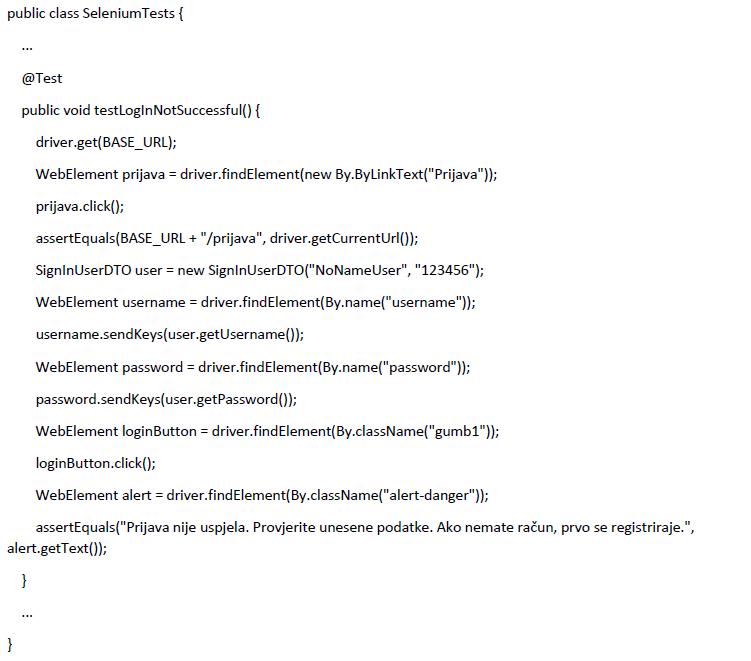
\includegraphics[scale=0.9]{slike/sel3.PNG} %veličina slike u odnosu na originalnu datoteku i pozicija slike
				\centering
				\caption{Testiranje prijave nepostojećeg korisnika}
				\label{fig:sel3}
			\end{figure}
			
			
			
			
			\textbf{Ispitni slučaj 4: Testiranje slanja poruka
				}
			Testiramo slanje poruka između dvaju postojećih korisnika. Prijavljujemo se na jedan korisnički račun (metoda login(String username, String password)), zatim šaljemo poruku korisiniku i odjavljujemo se kako bismo se mogli prijaviti na drugi korisnički račun. Nakon prijave korisnika koji je trebao zaprimiti poruku i provjeraamo postoji li poruka koju smo poslali.
			
			
			\begin{figure}[H]
				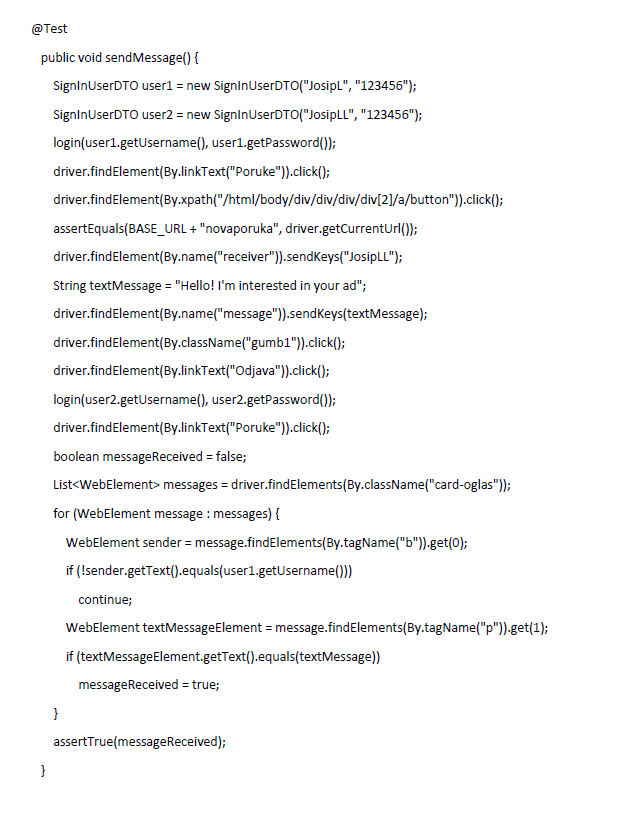
\includegraphics[scale=0.9]{slike/sel4.PNG} %veličina slike u odnosu na originalnu datoteku i pozicija slike
				\centering
				\caption{Testiranje slanja poruke}
				\label{fig:sel4}
			\end{figure}
			
			\textbf{Ispitni slučaj 5: Testiranje objave oglasa
				}
			
			Testiramo objavu oglasa tako s početne stranice te nakon toga provjeravamo je li se upravo objavljeni oglas pojavio u korisnikovoj listi njegovih objavljenih oglasa. 
			
			\begin{figure}[H]
				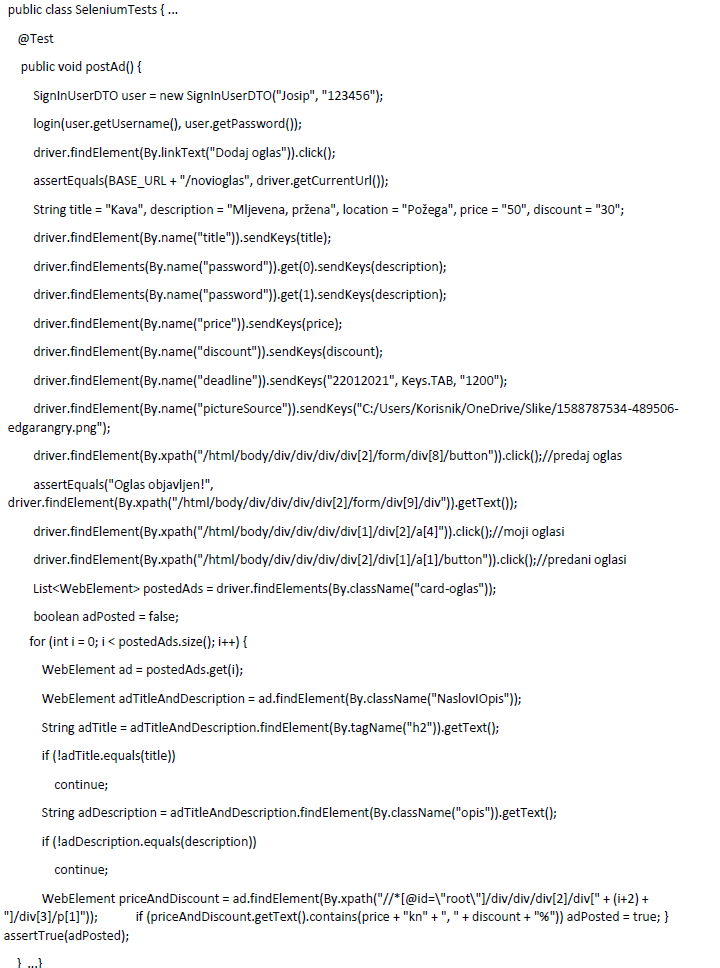
\includegraphics[scale=0.9]{slike/sel5.PNG} %veličina slike u odnosu na originalnu datoteku i pozicija slike
				\centering
				\caption{Testiranje objave oglasa}
				\label{fig:sel5}
			\end{figure}
			
			\eject 
			
			\section{Dijagram razmještaja}
		
		Dijagrami razmještaja opisuju topologiju sklopovlja i programsku potporu koja se koristi u implementaciji sustava u njegovom radnom okruženju. Na poslužiteljskom računalu se nalaze web poslužitelj i poslužitelj baze podataka. Klijenti koriste web preglednik kako bi pristupili web aplikaciji. Sustav je baziran na arhitekturi ”klijent – poslužitelj”, a komunikacija između računala korisnika (kupac, ponuđač, administrator) i poslužitelja odvija se preko HTTP veze. 
		
		\begin{figure}[H]
				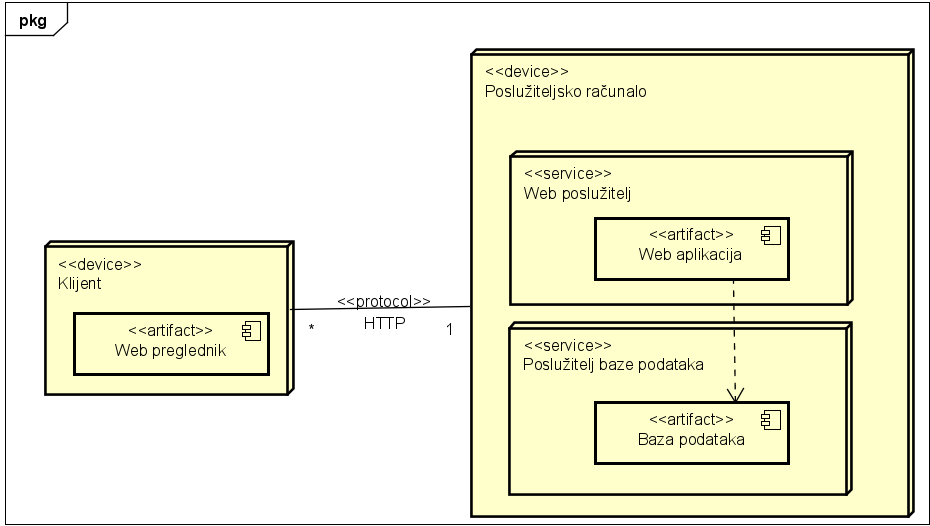
\includegraphics[scale=0.7]{slike/DijagramRazmjestaja.PNG} %veličina slike u odnosu na originalnu datoteku i pozicija slike
				\centering
				\caption{Dijagram razmještaja}
				\label{fig:java}
			\end{figure}
			
			\eject
			
		\section{Upute za puštanje u pogon}
		
			\textbf{\textit{Instalacija potrebnih aplikacija}}
			
			Za pokretanje ove aplikacije kao poslužitelja potrebno je imati instalirano nekoliko aplikacija koje omogućavaju pokretanje i sam rad aplikacije.
		
			Za bazu je potrebno instalirati pgAdmin koji omogućava povezivanje na PostgreSQL bazu podataka.Poveznica za preuzimanje je: \url{https://www.pgadmin.org/download/} ali se i u  popisu literature nalazi poveznica na kojemu je moguće preuzeti pgAdmin te postoje detaljne upute kako se može postaviti sve potrebno za rad baze.
		
			Na računalu je svakako potrebno imati podršku za prevođenje i pokretanje aplikacija napisanih u programskom jeziku Java. Također poveznica za preuzimanje potrebne podrške: \url{http://jdk.java.net/11/} te je dodana u popisu literature te se lako mogu pronaći upute koje će vas voditi kroz postavljanje svega potrebnog za uspostavu podrške za rad s programskim jezikom Java. Nakon instalacije je potrebno provjeriti radi li sve uspješno, a to je najjednostavnije provjeriti u naredbenom retku unosom naredbe "java -version". U danom primjeru je instalirana verzija 15, no za izvođenje programa je sasvim dovoljna verzija 11. 
			
			\begin{figure}[H]
				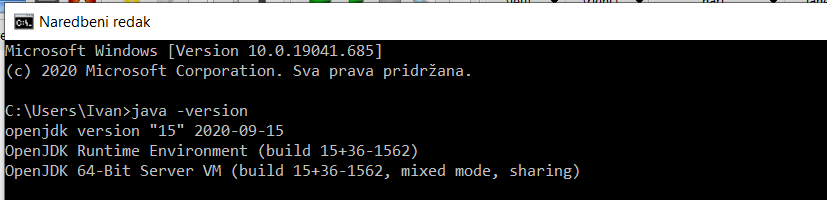
\includegraphics[scale=0.6]{slike/Java.PNG} %veličina slike u odnosu na originalnu datoteku i pozicija slike
				\centering
				\caption{Provjera instalacije Jave}
				\label{fig:java}
			\end{figure}
			
			Kako se uz Javu koristi i programski jezik JavaScript potrebno je instalirati i njegovu podršku odnosno potrebno je instalirati Node.js. Poveznica za instalaciju Node.js-a: \url{https://nodejs.org/en/download/} te je dana u popisu literature te se jednostavno uz pomoć uputa instalira. Također je potrebno provjeriti uspješnost instaliranja Node.js-a u naredbenom retku naredbom: " node -v".
			
			\begin{figure}[H]
				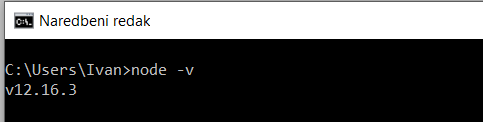
\includegraphics[scale=0.6]{slike/node.PNG} %veličina slike u odnosu na originalnu datoteku i pozicija slike
				\centering
				\caption{Provjera instalacije Node.js-a}
				\label{fig:node}
			\end{figure}
		
		Kada je sve to spremno potrebno je instalirati razvojnu okolinu koja nam pomaže pri izradi same aplikacije i njenog pokretanja. Primjer jedne takve okoline je Intelij IDE koji je za studente FER-a besplatan, no moguće je koristiti i druge razvojne okoline poput Eclipsa. Poveznica za preuzimanje ove razvojne okoline:  \url{https://www.jetbrains.com/idea/download/#section=windows}  također se nalazi i u popisu literature.
		
		Uz to za preuzimanje projekta možete se poslužiti sa Git GUI-em kojega je moguće preuzeti sa slijedeće poveznice: \url{https://git-scm.com/downloads}. Međutim možete samo skinuti projekt sa \url{https://gitlab.com/ivicamarica/ivicamarica} te ga pohraniti na željeno mjesto.
		
		Za kraj morate na svome računalu imati i program za upravljanje projektima, u ovom slučaju je to Gradle. \url{https://gradle.org/install/} je poveznica za prezimanje.
		
		Kada ste sve to pripremili konačno možete pokrenuti aplikaciju. Za uspješno pokretanje aplikacije potrebno je prvo instalirati npm pakete koji se koriste. To se treba učiniti pokretanjem naredbe
		npm install unutar direktorija src/main/js.
		Spring Boot aplikaciju je moguće pokrenuti unutar IDE-a ili naredbom gradle bootRun iz naredbenog retka.
		Frontend se pokreće naredbom npm start unutar direktorija src/main/js nakon čega se aplikacija može pregledavati u pregledniku na adresi http://localhost:3000.
		Nakon što ste ovako pokrenuli aplikaciju možete ju koristiti jer će se ona sama pobrinuti za sve potrebne komponente poput stvaranja baze i ostaloga.
		
		Ukoliko samo želite pogledati i isprobati aplikaciju, aplikacija je dostupna na poveznici  \url{https://progi-stop-waste.herokuapp.com/}.
		
		
		
		
			 
			
			\eject 
	%\chapter{Zaključak i budući rad}
		
		 \textit{Zadatak naše grupe bio je razvoj web aplikacije koja pridonosi smanjuje bacanje hrane, uz mogućnosti upravljanja rezervacijom, oglasima i porukama. Ostvarili smo zadani cilj nakon 15 tjedana rada u timu. Sama provedba projekta podjeljena je u dvije faze.}
		 
		 \textit{Prva faza projekta uključivala je okupljanje tima za razvoj aplikacije, dodjelu projektnog zadatka i intenzivan rad na dokumentiranju zahtjeva. Kvalitetna provedba prve faze uvelike je olakšala daljnji rad pri realizaciji osmišljenog sustava. Izrađeni obrasci i dijagrami (obrasci uporabe, sekvencijski dijagrami, model baze podataka, dijagram razreda) bili su od pomoći podtimovima zaduženima za razvoj backenda i frontenda. Izrada vizualnih prikaza idejnih rješenja problemskih zadataka uštedjela je mnogo vremena u drugom ciklusu kada su clanovi tima nailazili na nedoumice oko implementacije rješenja.}
		 
		 \textit{Druga faza ukazala je na manjak iskustva članova u izradi sličnih implementacijskih rješenja što je primorilo članove na samostalno učenje odabranih alata i programskih jezika. Osim realizacije rješenja, u drugoj fazi je bilo potrebno dokumentirati ostale UML dijagrame(dijagram stanja, dijagram aktivnosti, komponentni dijagram i dijagram razmještaja) i izraditi popratnu dokumentaciju kako bi budući korisnici mogli lakše koristiti ili vršiti preinake na sustavu. Komunikacija među članovima tima bila je putem Whatsappa i Microsoft Teamsa čime smo postigli informiranost svih članova grupe o napretku projekta. }
		 
		 \textit{OVDJE TREBA DODATI JOŠ FUNKCIONALNOSTI KOJA NISU IMPLEMENTIRANE U APLIKACIJI. Moguće proširenje postojeće inačice sustava je izrada mobilne aplikacije čime bi se cilj projektnog zadatka bio ostvaren u vecoj mjeri no s web aplikacijom.}
		 
		 \textit{Sudjelovanje na ovakvom projektu bilo je vrijedno iskustvo svim članovima tima jer smo iskusili rad u timu i stekli nova znanja u odabranim alatima i programskim jezicima. Takoder, osjetili smo važnost dobre vremenske organiziranosti i koordiniranosti između članova tima. Svakako bi s više iskustava članova tima otvarenje projekta bilo brže i kvalitetnije no unatoč tome zadovoljni smo s potignutignućem te ćemo u narednom periodu nastojat poboljšati funkcionalnosti aplikacije.}
		
		\eject 
	\chapter*{Popis literature}
		\addcontentsline{toc}{chapter}{Popis literature}
	 	
 		
		
		
		\begin{enumerate}
			
			
			\item  Programsko inženjerstvo, FER ZEMRIS, \url{http://www.fer.hr/predmet/proinz}
			
			\item  The Unified Modeling Language, \url{https://www.uml-diagrams.org/}
			
			\item  Astah Community, \url{http://astah.net/editions/uml-new}
			
			\item ERDPlus,
			\url{https://erdplus.com/}
			
			\item Slika StopWaste (pristupano 11.11.2020.), 
			\url{https://www.google.com/url?sa=i&url=http\%3A\%2F\%2Fwww.klexpatmalaysia.com\%2F2017\%2F02\%2F21\%2F5186\%2F&psig=AOvVaw2oATDkNqo4mue1uyCEpcFt&ust=1605218845441000&source=images&cd=vfe&ved=0CAIQjRxqFwoTCLj9wrDA--wCFQAAAAAdAAAAABAI
			}
		
			\item  pgAdmin,
			 \url{https://www.pgadmin.org/download/}
			 
			 \item  Java jdk 11,
			 \url{http://jdk.java.net/11/}
			 
			 \item  Node.js,
			 \url{https://nodejs.org/en/download/}
			 			 
			 \item  Inteliji IDE,
			 \url{https://www.jetbrains.com/idea/download/#section=windows}
			 
			 \item  Git,
			 \url{https://git-scm.com/downloads}
			 
			 \item  Gradle,
			 \url{https://gradle.org/install/}
			 
			 

			 
		
			
		\end{enumerate}
		
		 
	
	
	\begingroup
	\renewcommand*\listfigurename{Indeks slika i dijagrama}
	%\renewcommand*\listtablename{Indeks tablica}
	%\let\clearpage\relax
	\listoffigures
	%\vspace{10mm}
	%\listoftables
	\endgroup
	\addcontentsline{toc}{chapter}{Indeks slika i dijagrama}


	
	\eject 
		
	\chapter*{Dodatak: Prikaz aktivnosti grupe}
\addcontentsline{toc}{chapter}{Dodatak: Prikaz aktivnosti grupe}
		
		\section*{Dnevnik sastajanja}
		
		\begin{packed_enum}
			\item  sastanak
			
			\item[] \begin{packed_item}
				\item Datum: 29. rujna 2020.
				\item Prisustvovali: K.Mišura, I.Aradski, P.Brala, I.Fićković, J.Kolarec, J.Lukačević, A.Rakocija
				\item Teme sastanka:
				\begin{packed_item}
					\item  odabran voditelj tima i ime tima
					\item  odabrane pojedinosti za prijavu tima
				\end{packed_item}
			\end{packed_item}
			
			\item  sastanak
			\item[] \begin{packed_item}
				\item Datum: 7. listopada 2020.
				\item Prisustvovali:  K.Mišura, I.Aradski, P.Brala, J.Kolarec, J.Lukačević, A.Rakocija
				\item Teme sastanka:
				\begin{packed_item}
					\item  sastanak s asistenticom i demosom
					\item  raščišćavanje dilema funkcionalnosti 
					\item analiza zadatka
				\end{packed_item}
			\end{packed_item}
			
			\item sastanak
			\item[] \begin{packed_item}
				\item Datum: 8. listopada 2020.
				\item Prisustvovali:  K.Mišura, I.Aradski, P.Brala, I.Fićković, J.Kolarec, J.Lukačević, A.Rakocija
				\item Teme sastanka:
				\begin{packed_item}
					\item  procjena trajanja projekta
					\item  procjena znanja i sposobnsti članova
				\end{packed_item}
			\end{packed_item}
			
			\item  sastanak
			\item[] \begin{packed_item}
				\item Datum: 15. listopada 2020.
				\item Prisustvovali:  K.Mišura, I.Aradski, P.Brala, I.Fićković, J.Kolarec, J.Lukačević, A.Rakocija
				\item Teme sastanka:
				\begin{packed_item}
					\item  postavljanje gitlab repozitorija
					\item  konačan odabir alata i tehnologija  
				\end{packed_item}
			\end{packed_item}
			
			\item  sastanak
			\item[] \begin{packed_item}
				\item Datum: 19. listopada 2020.
				\item Prisustvovali:  K.Mišura, I.Aradski, P.Brala, I.Fićković, J.Kolarec, J.Lukačević, A.Rakocija
				\item Teme sastanka:
				\begin{packed_item}
					\item  pregled modela baze
					\item  pregled zamišljenog izgleda aplikacije 
				\end{packed_item}
			\end{packed_item}
			
			\item  sastanak
			\item[] \begin{packed_item}
				\item Datum: 22. listopada 2020.
				\item Prisustvovali:  K.Mišura, I.Aradski, P.Brala, I.Fićković, J.Kolarec, J.Lukačević, A.Rakocija
				\item Teme sastanka:
				\begin{packed_item}
					\item  ispravljanje pogrešaka u modelu baze podataka
				\end{packed_item}
			\end{packed_item}
			
			\item  sastanak
			\item[] \begin{packed_item}
				\item Datum: 28. listopada 2020.
				\item Prisustvovali:  K.Mišura, I.Aradski, P.Brala, I.Fićković, J.Kolarec, J.Lukačević, A.Rakocija
				\item Teme sastanka:
				\begin{packed_item}
					\item  podjela posla među članovima tima  
				\end{packed_item}
			\end{packed_item}
			
			\item  sastanak
			\item[] \begin{packed_item}
				\item Datum: 2. studenoga 2020.
				\item Prisustvovali:  K.Mišura, I.Aradski, P.Brala, I.Fićković, J.Kolarec, J.Lukačević, A.Rakocija
				\item Teme sastanka:
				\begin{packed_item}
					\item  postavljanje prvih uradaka na gitLab repozitorij 
				\end{packed_item}
			\end{packed_item}
			
			\item  sastanak
			\item[] \begin{packed_item}
				\item Datum: 3. studenoga 2020.
				\item Prisustvovali:  K.Mišura, I.Aradski, P.Brala, I.Fićković, J.Kolarec, J.Lukačević, A.Rakocija
				\item Teme sastanka:
				\begin{packed_item}
					\item  podjela uloga za rad na dokumentaciji 
				\end{packed_item}
			\end{packed_item}
			
			\item  sastanak
			\item[] \begin{packed_item}
				\item Datum: 9. prosinca 2020.
				\item Prisustvovali:  K.Mišura, I.Aradski, P.Brala, I.Fićković, J.Kolarec, J.Lukačević, A.Rakocija
				\item Teme sastanka:
				\begin{packed_item}
					\item  analiza projektnog zadatka 
					\item  podjela zadataka među članovima
				\end{packed_item}
			\end{packed_item}
			
			\item  sastanak
			\item[] \begin{packed_item}
				\item Datum: 20. prosinca 2020.
				\item Prisustvovali:  K.Mišura, I.Aradski, P.Brala, I.Fićković, J.Kolarec, J.Lukačević, A.Rakocija
				\item Teme sastanka:
				\begin{packed_item}
					\item  analiza projektnog zadatka 
					\item  pregled trenutno napravljenog
					\item  podjela zadataka među članovima
				\end{packed_item}
			\end{packed_item}
			
			\item  sastanak
			\item[] \begin{packed_item}
				\item Datum: 28. prosinca 2020.
				\item Prisustvovali:  K.Mišura, I.Aradski, P.Brala, I.Fićković, J.Kolarec, J.Lukačević, A.Rakocija
				\item Teme sastanka:
				\begin{packed_item}
					\item  analiza projektnog zadatka 
					\item  pregled trenutno napravljenog
					\item  podjela zadataka među članovima
					\item  dogovor oko izrade baze
				\end{packed_item}
			\end{packed_item}
			
			\item  sastanak
			\item[] \begin{packed_item}
				\item Datum: 29. prosinca 2020.
				\item Prisustvovali:  K.Mišura, I.Aradski, P.Brala, I.Fićković, J.Kolarec, J.Lukačević, A.Rakocija
				\item Teme sastanka:
				\begin{packed_item}
					\item  pregled izrađene baze
				\end{packed_item}
			\end{packed_item}
			
			\item  sastanak
			\item[] \begin{packed_item}
				\item Datum: 4. siječnja 2020.
				\item Prisustvovali:  K.Mišura, I.Aradski, P.Brala, I.Fićković, J.Kolarec, J.Lukačević, A.Rakocija
				\item Teme sastanka:
				\begin{packed_item}
					\item  analiza projektnog zadatka 
					\item  pregled trenutno napravljenog
					\item  pregled dokumentacije
					\item  podjela zadataka među članovima
					\item  podjela zadataka za izradu dokumentacije među članovima 
				\end{packed_item}
			\end{packed_item}
			
			\item  sastanak
			\item[] \begin{packed_item}
				\item Datum: 8. siječnja 2020.
				\item Prisustvovali:  K.Mišura, I.Aradski, P.Brala, I.Fićković, J.Kolarec, J.Lukačević, A.Rakocija
				\item Teme sastanka:
				\begin{packed_item}
					\item  demonstracija alfa verzije 
				\end{packed_item}
			\end{packed_item}
			%
			
		\end{packed_enum}
		
		\eject
		\section*{Tablica aktivnosti}
		
			
					
						
			
			\begin{longtabu} to \textwidth {|X[7, l]|X[1, c]|X[1, c]|X[1, c]|X[1, c]|X[1, c]|X[1, c]|X[1, c]|}
								
				\cline{2-8} \multicolumn{1}{c|}{\textbf{}} &     \multicolumn{1}{c|}{\rotatebox{90}{\textbf{Katarina Mišura }}} & \multicolumn{1}{c|}{\rotatebox{90}{\textbf{Igor Aradski }}} &	\multicolumn{1}{c|}{\rotatebox{90}{\textbf{Petra Brala }}} &	\multicolumn{1}{c|}{\rotatebox{90}{\textbf{Ivan Fićković }}} &
				\multicolumn{1}{c|}{\rotatebox{90}{\textbf{Josip Kolarec }}} &
				\multicolumn{1}{c|}{\rotatebox{90}{\textbf{Josip Lukačević }}} &	\multicolumn{1}{c|}{\rotatebox{90}{\textbf{Andrea Rakocija }}} \\ \hline 
				\endfirsthead
				
			
				\cline{2-8} \multicolumn{1}{c|}{\textbf{}} &     \multicolumn{1}{c|}{\rotatebox{90}{\textbf{Katarina Mišura}}} & \multicolumn{1}{c|}{\rotatebox{90}{\textbf{Igor Aradski }}} &	\multicolumn{1}{c|}{\rotatebox{90}{\textbf{Petra Brala }}} &
				\multicolumn{1}{c|}{\rotatebox{90}{\textbf{Ivan Fićković }}} &	\multicolumn{1}{c|}{\rotatebox{90}{\textbf{Josip Kolarec }}} &
				\multicolumn{1}{c|}{\rotatebox{90}{\textbf{Josip Lukačević }}} &	\multicolumn{1}{c|}{\rotatebox{90}{\textbf{Andrea Rakocija }}} \\ \hline 
				\endhead
				
				
				\endfoot
							
				 
				\endlastfoot
				
				Upravljanje projektom 		& 5 & 1 &  & 3  &  &  & \\ \hline
				Opis projektnog zadatka 	&  &  & 2 &  &  & 2 & \\ \hline
				
				Funkcionalni zahtjevi       &  & 2 &  &  &  &  &  \\ \hline
				Opis pojedinih obrazaca 	&  & 1 &  &  &  &  & 6 \\ \hline
				Dijagram obrazaca 			&  &  &  &  & 2  &  &  \\ \hline
				Sekvencijski dijagrami 		&  &  &  &  & 2 &  &  \\ \hline
				Opis ostalih zahtjeva 		&  &  &  &  &  &  &  \\ \hline

				Arhitektura i dizajn sustava	 & 6 & 10 &  & 1 &  &  &  \\ \hline
				Baza podataka				& 8 & 1 &  & 7  &  &  &   \\ \hline
				Dijagram razreda 			&  &  & 2 &  4&  &  &   \\ \hline
				Dijagram stanja				&  &  &  &  2&  &  &  \\ \hline
				Dijagram aktivnosti 		&  &  &  &  &  &  &  \\ \hline
				Dijagram komponenti			&  &  &  &  &  &  &  \\ \hline
				Korištene tehnologije i alati 		&  &  &  &  &  &  &  \\ \hline
				Ispitivanje programskog rješenja 	&  & 1  &  & 2 &  & 1 &  \\ \hline
				Dijagram razmještaja			&  &  &  &  &  &  &  \\ \hline
				Upute za puštanje u pogon 		&  & 1 &  & 4 &  &  &  \\ \hline 
				Dnevnik sastajanja 			& 4 &  &  & 1  &  &  &  \\ \hline
				Zaključak i budući rad 		&  &  &  &  &  &  &  \\  \hline
				Popis literature 			&  &  &  & 1 &  &  &  \\  \hline
				Izrada početne stranice		&  & 10 & 3 &  & 3 &  & 20 \\ \hline 
				Izrada baze podataka		&  & 1 &  &4  &  &  & \\ \hline 
				Spajanje s bazom podataka	&  & 5 &  & 3 &  &  &  \\ \hline
				Back end					&  & 35 & 4 & 1 &  & 6 &  \\  \hline
				 							&  &  &  &  &  &  &\\  \hline
				
				
			\end{longtabu}
					
					
		\eject
		


\end{document} %naredbe i tekst nakon ove naredbe ne ulaze u izgrađen dokument